
\hypertarget{introduction}{%
\section{Introduction}\label{introduction}}

The world is Big Data, and The Cloud is its landlord. It is our
responsibility to ferret it out of its primitive unknown, mine it,
harvest it, dump it by the tanker-truckful into great Data Lakes
overhung by computational Clouds to refine the Actionable Insights from
its desiccated husk. The Cloud promises us an infinite, seamless expanse
of Knowledge. If only we can harness the wily spray of our Organic
Content, filtering our every action, affection, and affiliation through
a thicket of algorithmically optimized platforms then The Cloud might
teach us enough about ourselves to finally be happy. Information by its
many names is the central quilting point for contemporary capitalism
(eg. see \cite{warkCapitalDeadThis2021} ), and like prior
assemblages of capital is thick with contradiction. It is historically
contingent and inevitable, material and transcendent, a concrete set of
technologies and techniques as well as a web of belief systems, power,
and \emph{dreams.} The Cloud now dreams of a great Knowledge Graph of
Everything, to Dissolve the Silos that keep the Bigness of Data from
teaching us all we could know. It tells us this is important for the
fate of humanity.

The Knowledge Graph of Everything and all that it promises is a mirage,
though. Its history is that of
``\href{https://en.wikipedia.org/wiki/Primitive_accumulation_of_capital}{primitive
accumulation}'' of informational capital, the widening of informational
asymmetries, and the logical conclusion of a model of digital serfdom
where we are promised glimpses of unimaginable computational power
through the pinhole lens of platforms for rent. With the enclosure of
the web nearly total, and our ability to imagine it in any other form
eclipsed, information conglomerates now position themselves as
information ``Infrastructures'' rather than mere Platforms \cite{barnsWhenWebBecame2020, plantinInfrastructureStudiesMeet2018} . The
politics, property and power relationships of the contemporary web
recede into the background of always-on elastic computation. Public
resources are rallied to build seemingly public data infrastructures to
feed far-flung facets of public life to systems built for decidedly
private profit. Aside from the pathological nature of the Knowledge
Graph of Everything as a colonial vision of all data being put in its
one True order, it \emph{is impossible} and \emph{won't work.} Instead,
by uncritically adopting the logic of The Cloud, governments and
academics will be led along by the nose just long enough to build
critical mass for an interlocking set of platforms that ratchet us ever
further into the captivity of surveillance.

Approaching the information-surveillance-platform archipelago through
knowledge graphs gives us an underexplored lens with which to understand
the politics of contemporary data infrastructures. Their
\protect\hyperlink{knowledge-graphs-a-backbone-in-the-surveillance-economy}{history},
the development from the liberatory ambitions of the
\protect\hyperlink{semantic-web-priesthoods}{Semantic Web} and
\protect\hyperlink{linked-data-platforms}{Linked Data} into the
\protect\hyperlink{knowledge-graphs-panoptica}{panoptical} data systems
of the surveillance economy, is rich with `paths not taken' from which
we can reimagine a future. Two contemporary projects from the National
Institutes of Health
(\protect\hyperlink{nih-the-biomedical-translator}{NIH}) and National
Science Foundation (\protect\hyperlink{nsf-open-knowledge-network}{NSF})
illustrate the ways our ambitions for public data infrastructures are
steered by the constraints of the cloud and the imminent capacity for
harm that poses. Rather than some obscure squabble between academics,
public knowledge graph projects intersect squarely with the
\protect\hyperlink{the-cloud-orthodoxy}{ideological foundation of The
Cloud} along with the parallel strains of ``AI'' to show how Large
Language Models (LLMs) are the tools for the next great
\protect\hyperlink{the-near-future-of-surveillance-capitalism-knowledge-graphs-get-chatbots.}{extension
of surveillance capitalism and re-entrenchment of informational
dominance}.

The past, present, and future of knowledge graphs give us the pieces to
articulate a properly \emph{human} data infrastructure as
\protect\hyperlink{vulgar-linked-data}{\textbf{vulgar linked data}}.
Predicated on relationality, heterogeneity, distribution of power, and
vernacular expression, vulgar linked data infrastructures attempt to
empower \emph{people} to \emph{socially organize} information in a truly
decentralized sociotechnological commons, rather than empowering
\emph{systems} to \emph{rent} knowledge organization for \emph{profit.}

\hypertarget{knowledge-graphs-a-backbone-in-the-surveillance-economy}{%
\section{Knowledge Graphs: A Backbone in the Surveillance
Economy}\label{knowledge-graphs-a-backbone-in-the-surveillance-economy}}

Knowledge graphs as a technology are relatively straightforward to
define \cite{chaudhriKnowledgeGraphsIntroduction2022, hitzlerReviewSemanticWeb2021, yanRetrospectiveKnowledgeGraphs2018, bergmanCommonSenseView2019}  (though see \cite{ehrlingerDefinitionKnowledgeGraphs2016} ): \textbf{directed, labeled
graphs} consisting of \emph{nodes} corresponding to entities like a
person, dataset, location, etc. and \emph{edges} that describe their
relationship\sidenote{Equivalently, one could emphasize that they are
  graphs composed of \textbf{triplet} links (or just \textbf{triplets})
  that describe some subject, predicate, and object.}. Knowledge graphs
typically make use of some controlled \textbf{ontology} that provides a
specific set of terms for nodes and edges and how they are to be used,
and ``types'' that give a given entity an expected set of
\emph{properties} represented by edges. This makes for an extremely
general data structure, where heterogeneous data can form a continuous
graph in a way that is both structured and can accommodate ad-hoc
modification not anticipated by a schema. For example, in Wikidata,
Peter Kropotkin (\href{https://www.wikidata.org/wiki/Q5752}{Q5752}) is
an \href{https://www.wikidata.org/wiki/Property:P31}{instance of} the
``\href{https://www.wikidata.org/wiki/Q5}{human}'' type, which
\href{https://www.wikidata.org/wiki/Property:P1963}{has properties} like
\href{https://www.wikidata.org/wiki/Property:P21}{\texttt{sex\ or\ gender}}
(\href{https://www.wikidata.org/wiki/Q6581097}{male}) and
\href{https://www.wikidata.org/wiki/Property:P19}{\texttt{place\ of\ birth}}
(\href{https://www.wikidata.org/wiki/Q649}{Moscow}), but also has
additional properties not in the \texttt{human} type like
\href{https://www.wikidata.org/wiki/Property:P109}{\texttt{signature}}.
Each of the ``edges'' like \texttt{place\ of\ birth} link to other nodes
like \texttt{Moscow}, which in turn have their own sets of links, and so
on.

Knowledge graphs are in themselves a fairly ordinary class of data
structures and technologies, but their history is the story of the
enclosure of the wild and open web into a series of surveillance-backed
platforms.

\hypertarget{semantic-web-priesthoods}{%
\subsection{Semantic Web:
Priesthoods}\label{semantic-web-priesthoods}}

The term ``Knowledge Graph'' evolved out of the Semantic Web project
\cite{hitzlerReviewSemanticWeb2021} , and so we rewind to the
start point of our history at the end of the 90's. It is difficult to
reconstruct how radical the notion of a collection of documents
organized by arbitrary links between them was at dawn of the internet.
At the time, the infrastructures of linking documents looked more like
ISBNs, carefully regulated by expert, centralized
authorities\sidenote{For another example re: the political nature of the
  DOI system in the face of the arbitrary linking of the internet, see
  \protect\hyperlink{ux201copenux201d-standards-are-yet-another-fraught-domain-of-openness-for}{section
  3.1 below} or section 3.1.2
  ``\href{https://jon-e.net/infrastructure/\#seemingly-prosocial-protocols-can-be-used-by-industries-to-preem}{Integration,
  not Invention}'' in \cite{saundersDecentralizedInfrastructureNeuro2022} }. Being able to
\emph{just link to anything} was \emph{terrifying} and \emph{new} (eg.
\cite{berners-leeLinksLaw1997, berners-leeLinksLawMyths1997} ).

The initial design of the web imagined it as a self-organizing process,
where people would maintain their own websites and organize a collection
of links to other websites\sidenote{For example, see the
  \href{http://meatballwiki.org/wiki/TourBusMap}{Tour Bus} system in
  early wikis, where each wiki would agree to link to the next wiki in
  the ``bus line,'' so someone that landed at the Meatball Wiki
  \href{http://meatballwiki.org/wiki/TourBusStop}{Bus Stop} and was
  interested in seeing ``eclectic'' wikis would continue on through (now
  defunct) WikiTravel and
  \href{http://toothycat.net/wiki/wiki.pl?TourBusStop}{ToothyWiki}.}. It
became clear relatively quickly that the anarchy of a socially
self-organizing internet wasn't going to work as planned, where without
a formal system of organization ``people were frightened of getting lost
in it. You could follow links forever.'' \cite{berners-leeWhatSemanticWeb1998} 

Like the radical nature of linking on the web, it's difficult to
remember that the web as surveillance apparatus thinly veiled as the
five or so remaining platform-websites was not inevitable. The
pre-dotcom bust internet of the 90's and early 2000's was far from the
commercialized wasteland we know today. Ed Horowitz, CEO of Viacom
explained in 1996: ``The Internet has yet to fulfill its promise of
commercial success. Why? Because there is no business model'' \cite{tarnoffInternetPeopleFight2022} . Google's AdWords being a defining
moment in the development of surveillance capitalism is a story already
told \cite{zuboffAgeSurveillanceCapitalism2019} : taking
advantage of the need for search generated by the disorganization of the
web, AdWords turned personal search data into a profit vector by selling
targeted space in the results.

The significance of the relationship between search, the semantic web,
and what became knowledge graphs is less widely appreciated. The
semantic web was initially an alternative to monolithic search engine
platforms - or, more generally, to platforms in general \cite{berners-leeSociallyAwareCloud2009} . It imagined the use of triplet
links and shared ontologies at a protocol level as a way of organizing
the information on the web into a richly explorable space: rather than
needing to rely on a search bar, one could traverse a structured graph
of information \cite{berners-leeLinkedData2006, berners-leeGoalsHumanDataInterface2010}  to find what one needed
without mediation by a third party.

The Semantic Web project was an attempt to supplement the arbitrary
power to express human-readable information in linked documents with
computer-readable information. It imagined a linked and overlapping set
of schemas ranging from locally expressive vocabularies used among small
groups of friends through globally shared, logically consistent
ontologies. The semantic web was intended to evolve fluidly, like
language, with cultures of meaning meshing and separating at multiple
scales \cite{berners-leeScalefreeNatureWeb1998, berners-leeSemanticWeb2001, berners-leeCulturesBoundaries2007} :

\begin{leftbar}
Locally defined languages are easy to create, needing local consensus
about meaning: only a limited number of people have to share a mental
pattern of relationships which define the meaning. However, global
languages are so much more effective at communication, reaching the
parts that local languages cannot. {[}\ldots{]}

So the idea is that in any one message, some of the terms will be from a
global ontology, some from subdomains. The amount of data which can be
reused by another agent will depend on how many communities they have in
common, how many ontologies they share.

In other words, one global ontology is not a solution to the problem,
and a local subdomain is not a solution either. But if each agent has
uses a mix of a few ontologies of different scale, that is forms a
global solution to the problem. \cite{berners-leeScalefreeNatureWeb1998} 
\end{leftbar}

\begin{leftbar}
The Semantic Web, in naming every concept simply by a URI, lets anyone
express new concepts that they invent with minimal effort. Its unifying
logical language will enable these concepts to be progressively linked
into a universal Web. \cite{berners-leeSemanticWeb2001} 
\end{leftbar}

This free form goal of expression for expression's sake was always in
tension with another part of the vision - serving as a backbone for AI
``agents'' that could compute emergent function from the semantic web.
Succinctly: ``Human language thrives when using the same term to mean
somewhat different things, but automation does not.'' \cite{berners-leeSemanticWeb2001}  This tension persists through the
broader history of the web, and
\protect\hyperlink{the-near-future-of-surveillance-capitalism-knowledge-graphs-get-chatbots.}{we
will return to it soon}.

\hypertarget{linked-data-platforms}{%
\subsection{Linked Data: Platforms}\label{linked-data-platforms}}

Much of the work of the semantic web project in the early 2000s focused
on the ``global'' side of this tension at the expense of the ``local'' -
creating ontologies and related technologies intended to serve as a
foundation for expressing basic things in a common vocabulary \cite{hitzlerReviewSemanticWeb2021} . This work had many successes, but
began a schism between the priesthood of people concerned with making
systems that were \emph{correct} and those that were more concerned with
making things that \emph{worked} - or supported ``local'' expression (eg
\cite{palmerDitchingSemanticWeb2008} ). Aaron Swartz captured
this frustration in his unfinished book:

\begin{leftbar}
Instead of the ``let's just build something that works'' attitude that
made the Web (and the Internet) such a roaring success, they brought the
formalizing mindset of mathematicians and the institutional structures
of academics and defense contractors. They formed committees to form
working groups to write drafts of ontologies that carefully listed (in
100-page Word documents) all possible things in the universe and the
various properties they could have, and they spent hours in Talmudic
debates over whether a washing machine was a kitchen appliance or a
household cleaning device. \cite{swartzAaronSwartzProgrammable2013} 
\end{leftbar}

Lindsay Poirier describes this difference in ``thought styles'' as a
rift between the ``neats'' focused on universalizing \emph{a priori}
ontologies and the ``scruffies'' focused on everyday use and letting the
structure appear afterwards \cite{poirierTurnScruffyEthnographic2017} . The latter characterizes the ``second age'' of the Semantic Web
after 2006 - the reorganization around \textbf{Linked Data} \cite{berners-leeLinkedData2006, hitzlerReviewSemanticWeb2021} . The era of
Linked Data de-emphasized the idealistic and ideological goals of the
early Semantic Web, driven more by an empirical approach of trying to
realize these systems on the wilds of the web, creating some of the
first public ``Linked Open Data'' systems like DBPedia and Freebase.

This turn coincides with the emerging platformatization and enclosure of
the web as ``Web 2.0.'' Throughout the early 2000s, the work of the
Semantic Web project was largely invisible to the ordinary web user, and
its vision of a self-organizing web was easily outcompeted by the
now-ubiquitous use of search engines to index the web. Where in the
early 2000s web architects were imagining the future of web continuing
to take place on free and open \emph{protocols,} the Linked Data/Web 2.0
era corralled us into a pattern of \emph{platforms} which quickly
ratcheted their way to dominance in a positive feedback loop of user
experience design, network effects, and profit. On platforms, rather
than a system that ``belongs'' to everyone, you are granted access to
some specific set of operations through an interface so that you can be
part of a social process of producing and curating information for the
platform holder. Shifting focus from the idealistic vision of public,
protocol-driven self-organization to platforms for declaring and
consuming semantic web data resulted in a lot of functional tools, but
also ripened the project for capture.

\hypertarget{knowledge-graphs-panoptica}{%
\subsection{Knowledge Graphs:
Panoptica}\label{knowledge-graphs-panoptica}}

In 2010 Google acquired Metaweb and its publicly-edited Semantic Web
database Freebase, and in 2012 repackaged it and the ideas of Linked
Data as what it called a \textbf{Knowledge Graph} --- the third era of
the Semantic Web \cite{singhalIntroducingKnowledgeGraph2012, iainFreebaseDeadLong2016} . Freebase only made up part of it, and the
full extent of Google's Knowledge Graph is unknown, but its most visible
impact are the factboxes that present structured information about the
subjects of searches - like biographical information in a search for a
person, or the different widgets for contextual interaction like
restaurant reservations\sidenote{The imagination of the bored, middle
  class platform developer seems to be populated primarily by ordering
  food from restaurants and shopping.} \cite{noyIndustryscaleKnowledgeGraphs2019} . Knowledge Graphs still share
the same underlying structure --- triplet graphs with ontologies ---
even if they occupy a broader space of implementations and technologies.
What differs is the context and intended use: the ``worldview'' of the
knowledge graph.

Beyond the obvious product-level features it supports, Google's
acquisition of Freebase and the structure of its Knowledge Graph
represent at least two deeper shifts in the trajectory of the Semantic
Web and the broader internet: the privatization of technologies with
initially liberatory aspirations, and an early template of the all too
familiar sprawling, surveillance-driven information conglomerate.

The form of of the semantic web that emerged as ``Knowledge Graphs''
flipped the vision of a free and evolving internet on its head. The
mutation from ``Linked Open Data'' \cite{berners-leeLinkedData2006}  to ``Knowledge Graphs'' is a shift in meaning from a public and
densely linked web of information from many sources to a proprietary
information store used to power derivative platforms and services. The
shift isn't quite so simple as a ``closure'' of a formerly open resource
--- we'll return to the complex role of openness in a moment. It is
closer to an \emph{en}closure, a \emph{domestication} of the dream of
the Semantic Web. A dream of a mutating, pluralistic space of
communication, where we were able to own and change and create the
information that structures our digital lives was reduced to a ring of
platforms that give us precisely as much agency as is needed to keep us
content in our captivity. Links that had all the expressive power of
utterances, questions, hints, slander, and lies were reduced to mere
facts. We were recast from our role as \emph{people} creating a digital
world to \emph{consumers} of subscriptions and services. The artifacts
that we create for and with and between each other as the substance of
our lives online were yoked to the acquisitive gaze of the knowledge
graph as \emph{content} to be mined. We vulgar commoners, we data
subjects, are not allowed to touch the graph --- even if it is built
from our disembodied bits.

The same technologies, with minor variation, that were intended to keep
the internet free became emblematic of and coproductive with the
surveillance/platform model that has enclosed it. Beyond Google,
knowledge graphs are an elemental part of the information economy.
Banks, militaries, governments, life science corporations, journalists,
everyone is using knowledge graphs \cite{neo4jNeo4jCustomers, enterpriseknowledgegraphfoundationKnowledgeGraphIndustry2022} . Their
ubiquity is not an accident, one of many possible data systems that
could have fit the bill, but reflects and reinforces basic patterns of
the information economy and the corporations within it. Conveniently,
semantic web technologies, designed to accommodate the infinitely
heterogeneous, multiscale nature of free and unmediated social
structuring of information are also quite useful for the indefinitely
expanding dragnet of data collection that defines the operation of
contemporary capitalism.

Data companies --- most major companies\sidenote{\begin{leftbar}
  ``If one takes a look at the top Fortune 500 companies, it is
  surprising how many of them are really in the information business. I
  don't just mean the technology and telecommunication companies like
  Apple or Google or Verizon or Cisco or the drug companies like Pfizer.
  One could also think of the big banks as a subset of the vectoralist
  class rather than as ``finance capital.'' They too are in the
  information asymmetry business. And as we learned in the 2008 crash,
  even the car companies are in the information business---they made
  more money from car loans than cars. The military---industrial sector
  is also in the information business. The companies that appear to sell
  actual things, like Nike, are really in the brand business. Walmart
  and Amazon compete with different models of the information logistics
  business. Even the oil companies are in part at least in the
  information-about-the-geology-of-possible-oil-deposits business.
  Perhaps the vectoralist class is no longer emerging. Maybe it is the
  new dominant class.'' \cite{warkCapitalDeadThis2021} 
  \end{leftbar}} --- need to store and maintain massive collections of
heterogeneous data across their byzantine hierarchies of executives,
managers, and workers. This gigantic haunted ball of data is not just a
tool, but the \emph{substance} of the company. A data company persists
by exploiting the combinatorics of its data hoard, spinning off new
platforms that in turn maintain and expand access to data by creating
captive data subjects\sidenote{Facebook describes its platform as being
  just a means of interacting with its underlying data graph in the
  jargon of corporate web design: ``A useful tool for Facebook has been
  to think of the graph as the model and a Facebook page as the view---a
  projection of an entity or collection of entities that reside in the
  graph.'' \cite{noyIndustryscaleKnowledgeGraphs2019} }. As it
expands, a conglomerate will acquire many new sources and modalities of
data and need to integrate them with its existing data.

Knowledge graphs are particularly well suited for this ``data
integration'' problem. A full technical description is out of scope
here, but briefly: traditional relational database systems can be very
difficult to modify and refactor, and that difficulty increases the
larger and more complex a database is\sidenote{For a practical example,
  see a recent
  \href{https://www.etsy.com/codeascraft/scaling-etsy-payments-with-vitess-part-1--the-data-model}{trio}
  of
  \href{https://www.etsy.com/codeascraft/scaling-etsy-payments-with-vitess-part-2--the-seamless-migration}{blog}
  \href{https://www.etsy.com/codeascraft/scaling-etsy-payments-with-vitess-part-3--reducing-cutover-risk}{posts}
  from Etsy engineers that describe the process of scaling their
  database system.}. One has to design the structure of the anticipated
data in advance, and the abstract schematic structure of the data is
embedded in how it is stored and accessed. It is particularly difficult
to do unanticipated ``long range'' analyses where very different kinds
of data are analyzed together.

In contrast, merging graphs is more straightforward\sidenote{\begin{leftbar}
  That is because knowledge graphs aim to solve the data incongruence
  problem, which is one of the biggest operational headaches for
  corporates, says Atkin. ``Corporates suffer from technology
  fragmentation and as a result have a lot of data that doesn't align
  across the organization. Doing the hard work to fix this data
  incongruence reality is a pre-requisite for realizing business
  value,'' he says. \cite{schenkerNewReportDetails2021} 
  \end{leftbar}} \cite{chaudhriKnowledgeGraphsIntroduction2022, enterpriseknowledgegraphfoundationKnowledgeGraphIndustry2022, schenkerNewReportDetails2021, sequedaDesigningBuildingEnterprise2021, azziniAdvancesDataManagement2021, segaranTwophaseConstructionData2020, ceravoloBigDataSemantics2018, natarajanGraphKnowledgeGraph}  - the
data is just triplets, so in an idealized case\sidenote{I am aware graph
  databases are not magic and this is an extraordinarily simplified
  example. The principle is the point, not all the subtle ways the
  implementations of graph databases are hard.} it is possible to just
concatenate them and remove duplicates (eg. for a short example, see
\cite{allemangMergingDataGraphs2022, allemangMergingTablesHard2022} ). The graph can be operated on locally, with more global
coordination provided by ontologies and schemas, which themselves have a
graph structure \cite{villazon-terrazasKnowledgeGraphFoundations2017} . Discrepancies between graphlike schema can be resolved by, you
guessed it, making more graph to describe the links and transformations
between them. Long-range operations between data are part of the basic
structure of a graph - just traverse nodes and edges until you get to
where you need to go - and the semantic structure of the graph provides
additional constraints to that traversal. Again, a technical description
is out of scope here, graphs are not magic, but they are well-suited to
merging, modifying, and analyzing large quantities of heterogeneous
data\sidenote{Another way of looking at the capacity for heterogeneity
  in triplet graphs is by thinking of links as statements:
  \begin{leftbar} One person may define a \texttt{vehicle} as having a
  \texttt{number\ of\ wheels} and a \texttt{weight} and a
  \texttt{length}, but not foresee a \texttt{color}. This will not stop
  another person making the assertion that a given car is \texttt{red},
  using the color vocabulary from elsewhere. \cite{berners-leeWhatSemanticWeb1998} \end{leftbar}}.

So if you are a data broker, and you just made a hostile acquisition of
another data broker who has additional surveillance information to fill
the profiles of the people in your existing dataset, you can just stitch
those new properties on like a fifth arm on your nightmarish data
Frankenstein.

\begin{center}\rule{0.5\linewidth}{0.5pt}\end{center}

What does this look like in practice? While in a bygone era Elsevier was
merely a rentier holding publicly funded research hostage for profit,
its parent company RELX is paradigmatic of the transformation of a more
traditional information rentier into a sprawling, multimodal
surveillance conglomerate (see \cite{lamdanDataCartelsCompanies2023} ). RELX proudly describes itself as a gigantic haunted graph of
data (Fig. \ref{fig:relx}):

\begin{leftbar}
Technology at RELX involves creating actionable insights from big data
-- large volumes of data in different formats being ingested at high
speeds. We take this high-quality data from thousands of sources in
varying formats -- both structured and unstructured. We then extract the
data points from the content, link the data points and enrich them to
make it analysable. Finally, we apply advanced statistics and
algorithms, such as machine learning and natural language processing, to
provide professional customers with the actionable insights they need to
do their jobs.

We are continually building new products and data and technology
platforms, re-using approaches and technologies across the company to
create platforms that are reliable, scalable and secure. \textbf{Even
though we serve different segments with different content sets, the
nature of the problems solved and the way we apply technology has
commonalities across the company.} \cite{relxAnnualReport20222023} 
\end{leftbar}

\begin{figure}[h!]
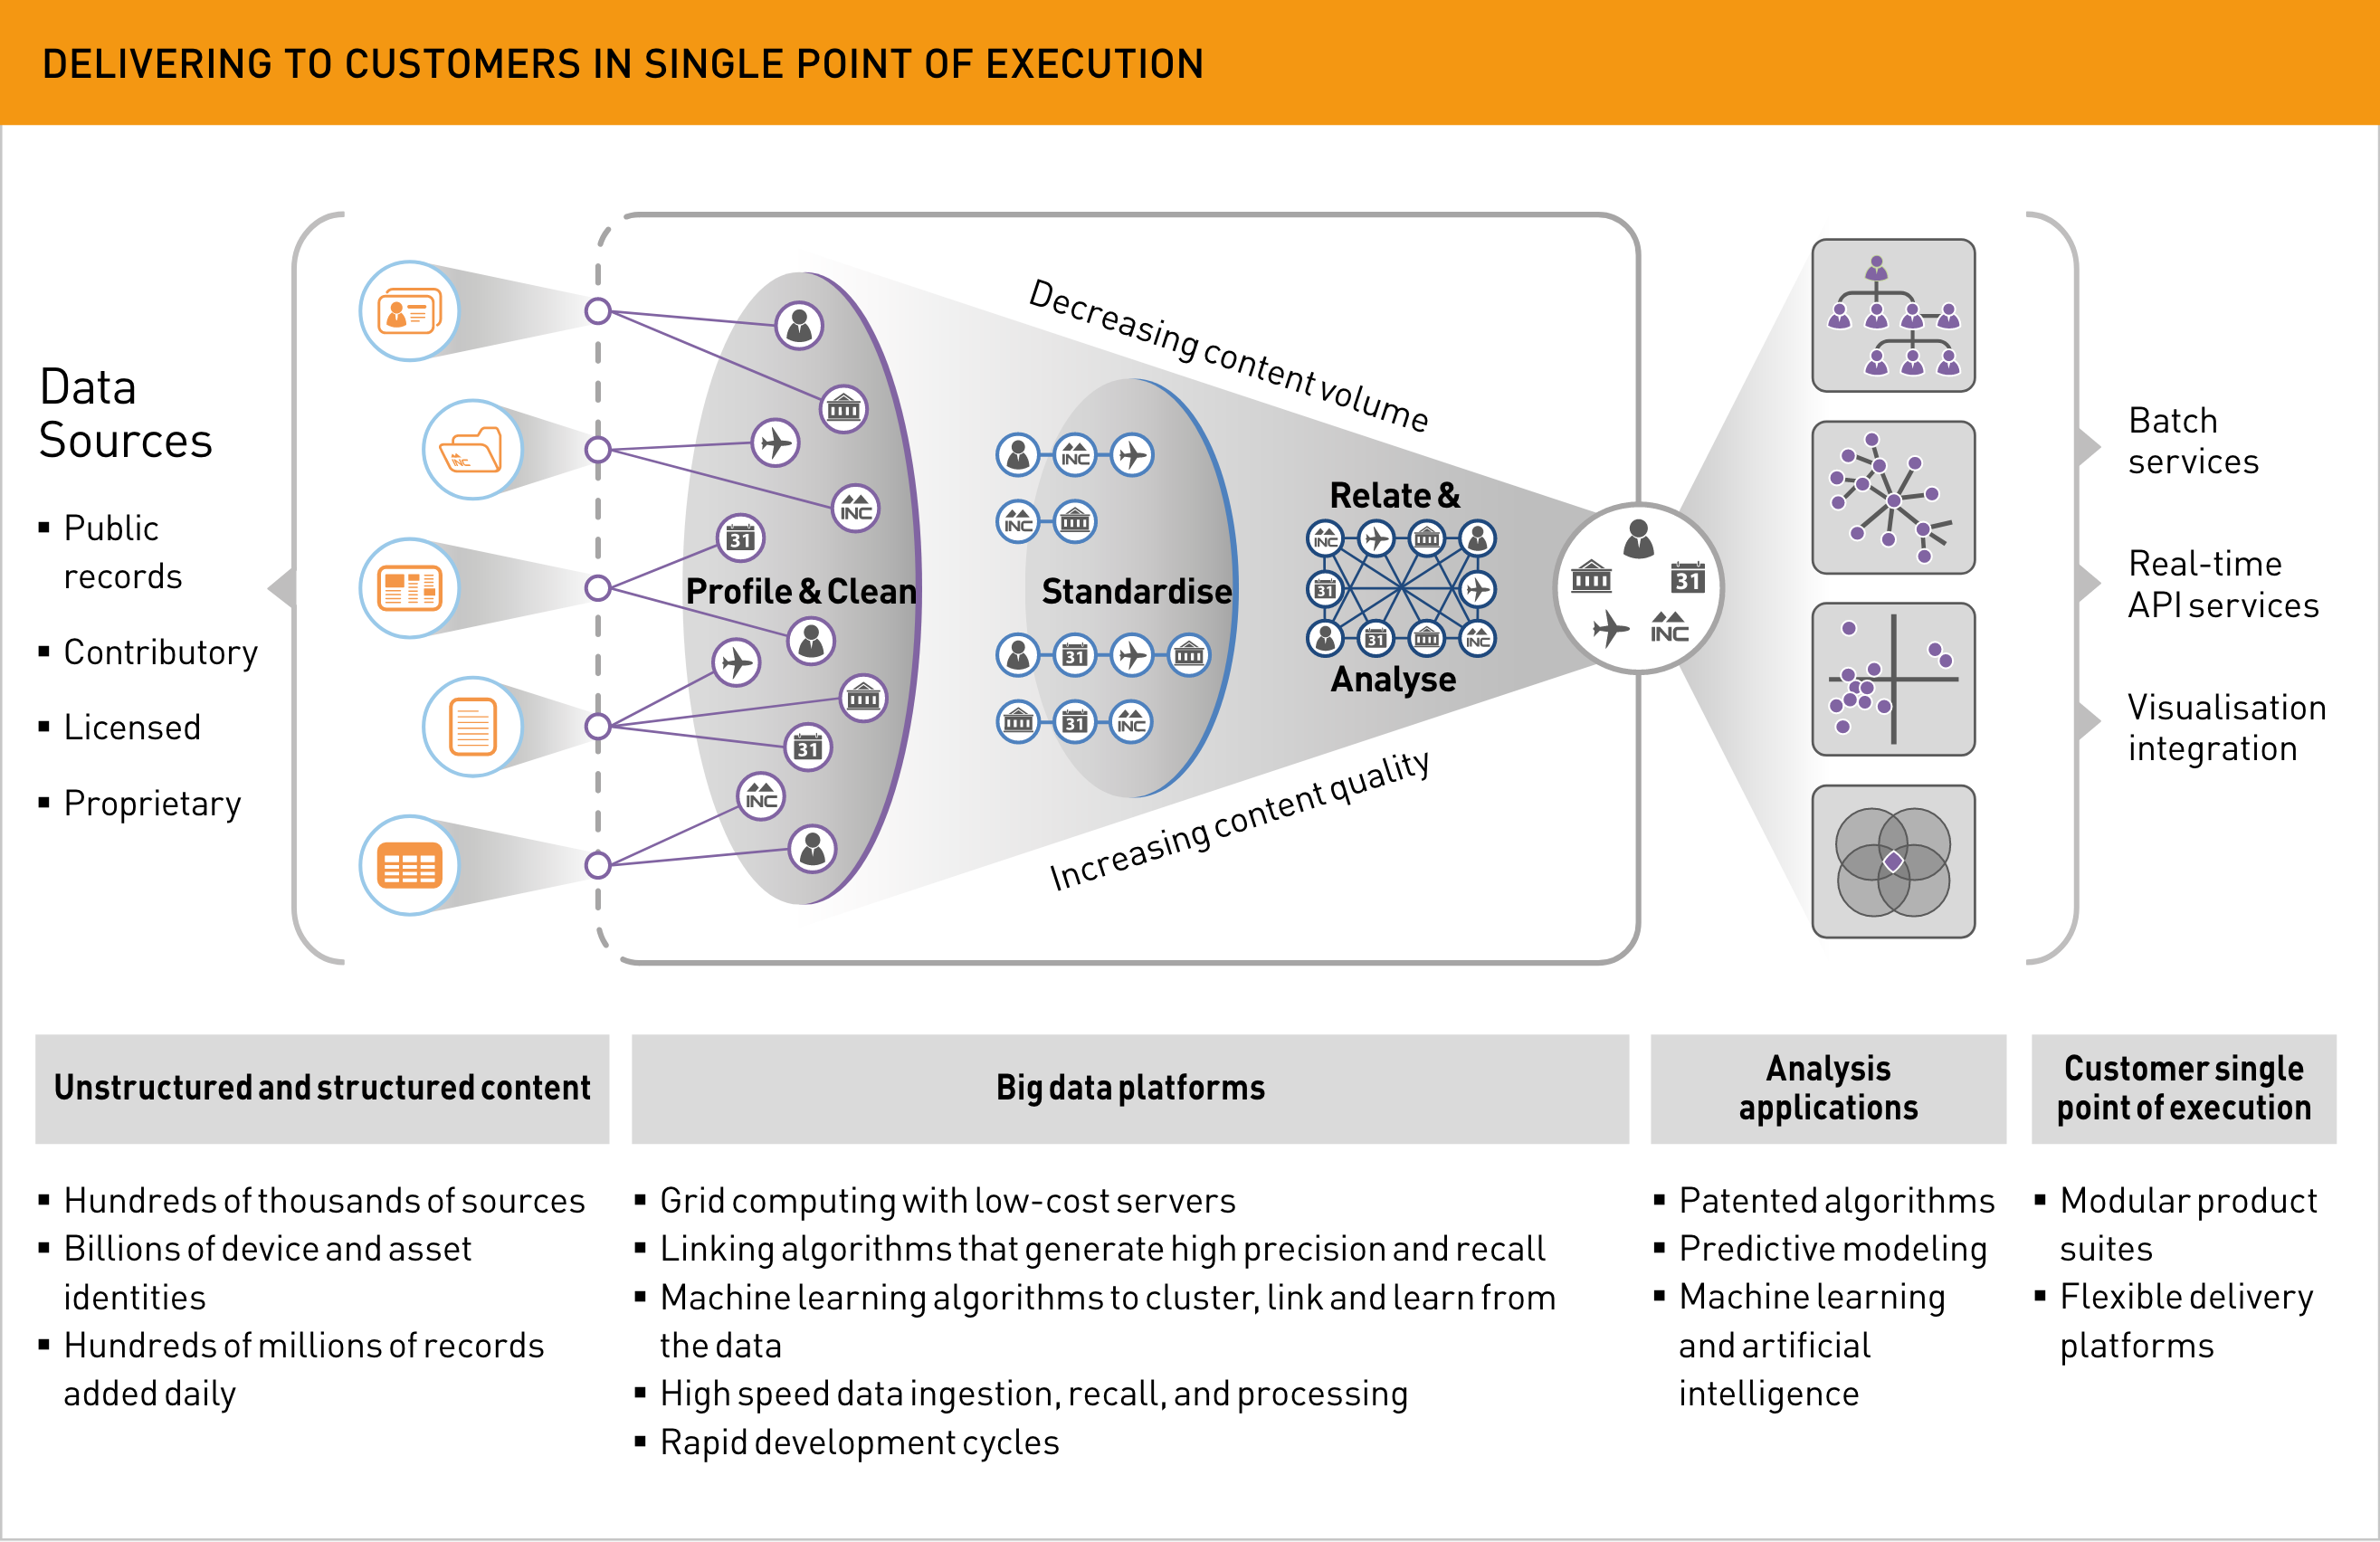
\includegraphics[width=\linewidth]{img/RELX_Pipeline_2022.png}

\caption{In its 2022 Annual Report, RELX describes its business model as
ingesting large quantities of data, linking them together, and deriving
platforms from them. \cite{relxAnnualReport20222023} }
\label{fig:relx}
\end{figure}

While to any individual market segment or class of customers RELX and
its subsidiaries might look like a portfolio of separate platforms and
applications, one can only make sense of the company by thinking of each
of them as a view on an interconnected graph of data\sidenote{Though
  apparently they have had historical difficulty actually getting that
  integration to work \cite{schonfeldReorganizationElsevier2022}.}. Each additional source of data, either by acquiring new
companies or by expanding their existing control of informational access
points has the potential to create some combinatorically new set of
opportunities for new platforms.

For example, RELX is able to gather surveillance data on researcher
attention data through the tracking in its ScienceDirect and Mendeley
platforms. It also collects a large amount of chemical data through its
control of scientific publishing that it rents access to on its
\href{https://www.elsevier.com/en-gb/solutions/reaxys}{Reaxys} platform,
which is supplemented by its LexisNexis (another RELX subsidiary)
PatentSight database of patents. So far so normal.

What about the other sides of the multisided market? RELX is able to
combine these and other data sources into new product. For
pharmaceutical R\&D companies, their bespoke
\href{https://web.archive.org/web/20211207070524/https://www.elsevier.com/solutions/professional-services/drug-design-optimization}{Drug
Design Optimization} services advertise being able to use chemical,
disease, and literature-based data to generate a priority list of
potential therapeutic targets and drugs, as well as provide
``competitive intelligence'' about which targets are currently being
studied, presumably identified from their ownership of the scientific
literature coupled with surveillance data. Since clinicians don't trust
pharmaceutical advertisements \cite{elsevierMakingMedicalInformation2021} , Elsevier uses its position as
a perceived neutral third party to repackage advertisements as
informational systems \cite{elsevierRethinkClincalContent2020} ,
``journal-branded webinars,'' as well as a number of other avenues via
its
``\href{https://web.archive.org/web/20211111211058/https://www.elsevier.com/advertising-reprints-supplements/advertising}{360
degree advertising solutions}'' catalogue. So, by combining several data
sources and platforms, Elsevier is able to offer pharmaceutical
companies recommendations for candidate drugs above and beyond what
would be possible with chemical information alone and then advertise
their drugs directly to doctors.

Derivative platforms beget derivative platforms, as each expands the
surface of dependence and provides new opportunities for data to
capture. Its integration into clinical systems by way of reference
material is growing to include
\href{https://web.archive.org/web/20230307020432/https://www.elsevier.com/en-gb/clinical-solutions/clinical-practice}{electronic
health record} (EHR) systems, and they are ``developing clinical
decision support applications {[}\ldots{]} leveraging {[}their{]}
proprietary health graph'' \cite{relxAnnualReport20222023} .
Similarly, their integration into Apple's watchOS to track medications
indicates their interest in directly tracking personal medical data.

That's all within biomedical sciences, but RELX's risk division also
provides ``comprehensive data, analytics, and decision tools for
{[}\ldots{]} life insurance carriers'' \cite{relxAnnualReport20222023} , so while we will never have the kind of
external visibility into its infrastructure to say for certain, it's not
difficult to imagine combining its diverse biomedical knowledge graph
with personal medical information in order to sell risk-assessment
services to health and life insurance companies. LexisNexis has personal
data enough to serve as an ``integral part'' of the United States
Immigration and Customs Enforcement's (ICE) arrest and deportation
program \cite{biddleLexisNexisProvideGiant2021, biddleICESearchedLexisNexis2022} , including dragnet
\href{https://web.archive.org/web/20230308034123/https://risk.lexisnexis.com/products/accurint-trax}{location
data} \cite{lexisnexisrisksolutionsAccurintTraX} ,
\href{https://risk.lexisnexis.com/products/telematics-ondemand}{driving
behavior data} from internet-connected cars \cite{lexisnexisrisksolutionsTelematicsOnDemand} , and
\href{https://risk.lexisnexis.com/products/threatmetrix}{payment and
credit data} as just a small sample from its large
\href{https://web.archive.org/web/20230308034302/https://www.lexisnexis.com/pdf/AccurintForLegalProfessionals/24.pdf}{catalogue}
\cite{lexisnexisrisksolutionsAccurintLegalProfessionals2022}  of
data \href{https://risk.lexisnexis.com/our-technology/lexid}{aggregated
and linked} into comprehensive profiles \cite{lexisnexisrisksolutionsLexID} . The contemporary knowledge
graph-powered surveillance conglomerate gains its versatility precisely
from its ability to span many unrelated domains and deploy new platforms
as opportunities present themselves. As new data sources are acquired,
the combinatorics of possible surveillance products correspondingly
explode.

This pattern is true across the information industry \cite{sequedaDesigningBuildingEnterprise2021} . A handful of
representatives from Microsoft, Google, Facebook, eBay, and IBM describe
some elements of each of their knowledge graphs in a 2019 paper \cite{noyIndustryscaleKnowledgeGraphs2019} . Each has different
scopes, applications, and interaction with the other data and processing
infrastructure at the company, but all emphasize the ability for their
knowledge graphs to accommodate change, heterogeneity, conflicting data,
inference, and facilitate work by distributed teams due to their
self-documenting and modular nature. Neo4j, developers of an eponymous
graph database library, describes in one
\href{https://neo4j.com/case-studies/us-army/}{case study} among its
\href{https://neo4j.com/customers/}{hundreds of customers} how the U.S.
Army uses its ``connected data'' to track its equipment and estimate the
cost of some new exploratory imperialism \cite{neo4jNeo4jArmyCase2021} . An analysis of Palantir's hundreds of
patents for knowledge graph technology (eg. \cite{cohenSystemMethodSharing2015, mathuraAutomatedDatabaseAnalysis2017, yousafSystemsMethodsUser2018, knudsonSystemsMethodsAnnotating2021} )
describes its ambitions for its knowledge graph:

\begin{leftbar}
There is evidence {[}\ldots{]} that Palantir has infrastructural
aspirations to become a general classification system for data
integration {[}\ldots{]} that can be tailored into a universal knowledge
graph. {[}\ldots{]} Palantir similarly imagines a world where its
platform might serve as a ``shadow'' universal knowledge graph for
governments, industries, and organizations. \cite{iliadisSeerSeenSurveying2022} 
\end{leftbar}

Knowledge graphs \emph{as a technology} - like all technologies - are
not intrinsically unethical. It is the structure of the capital-K
capital-G Knowledge Graph in its particular construction as a set of
property and power relationships set against the context of the platform
web that is pathological. They represent the historical trajectory of
semantic web ideas and technologies from something that we are intended
to use and create directly into privately held data that we can only
interact with through platforms. They are coproductive with the
corporate and technical structure of surveillance capitalism,
facilitating conglomerates that gobble up as many platforms and data
sources as possible to stitch them into an expanding, heterogeneous
graph of data.

In particular, it is their ``graph plus compute'' structure - where some
underlying graph of data is coupled with a set of algorithms and
interfaces to view it - that is necessary to understand some of the more
counterintuitive motivations of surveillance conglomerates. This
structure complicates questions of ``openness'' versus
``proprietariness,'' and provides a different lens on ostensibly
``open'' or ``public'' knowledge graph-based infrastructure projects.

\hypertarget{public-graphs-private-profits}{%
\section{Public Graphs, Private
Profits}\label{public-graphs-private-profits}}

\hypertarget{unqualified-openness-considered-harmful}{%
\subsection{Unqualified Openness Considered
Harmful}\label{unqualified-openness-considered-harmful}}

If the problem is information conglomerates stockpiling a massive
quantity of proprietary data and renting use of it, isn't ``open data''
the answer? ``Openness,'' including open source, open standards, and
open data, is a subtle tool that can be used both to dissolve and
reinforce economic and political power and is particularly ill-suited as
a counter-strategy for corporate knowledge graphs .

Free and open source software, with its noble (and decidedly
non-monolithic \cite{liuFreedomIsnFree2018} ) goal of creating an
ecosystem of free\sidenote{``free as in whatever will prevent you from
  @'ing me about getting some definition of free wrong.''} software, is
a means by which large information companies can harvest the commons and
outsource labor costs \cite{warkHackerManifesto2004, goldsmithOriginalSinFree2019, hallidayOpenSourceNot2018, hunterReclaimingComputingCommons2016, hornPostOpenSource2020} . There
are countless examples of FOSS developers maintaining software widely
used by companies making billions of dollars for little or no
compensation - eg.
\href{https://github.com/zloirock/core-js/blob/master/docs/2023-02-14-so-whats-next.md}{core-js}
\cite{pushkarevWhatNext2023} ,
\href{https://veridicalsystems.com/blog/of-money-responsibility-and-pride/index.html}{OpenSSL}
\cite{marquessSpeedsFeedsMoney2014} , leftpad \cite{gallagherRagequitCoderUnpublished2016} ,
\href{https://github.com/chrisdutz/blog/blob/main/plc4x/free-trial-expired.adoc}{PLC4X}
\cite{dutzYourFreeTrial2022}  and so on. When an information
company releases or supports an open source project it is rarely an act
of altruism. The effect is to prevent another company from profiting
from a proprietary version of that technology, signal virtue, drive
recruitment, and create a centralized point to concentrate donated
labor. Microsoft, a famously
\href{https://en.wikipedia.org/wiki/Embrace,_extend,_and_extinguish}{good
actor} in software, took this several steps further with GitHub, VSCode,
and later Copilot, capturing a large chunk of the software development
\emph{process} in order to trick programmers to be the
``\href{https://twitter.com/json_dirs/status/1410897161277956097}{humans
in the loop}'' refining the neural network to write code and dilute
their labor power \cite{butterickGitHubCopilotInvestigation2022, butterickGitHubCopilotLitigation2022, olearyVSCodeWhat2022, VSCodiumOpenSource} .

``\href{https://en.wikipedia.org/wiki/Peer_production}{Peer
production}'' models, a more generic term for public collaboration that
includes FOSS, has similar discontents. The related term
``crowdsource\sidenote{For critical work on crowdsourcing in the context
  of ``open science,'' see \cite{mirowskiFutureOpenScience2018} ,
  and in the semantic web see \cite{allhutterWorkingOntologistsHighQuality2019} .}'' quite literally
describes a patronizing means of harvesting free labor via some
typically gamified platform. Wikipedia is perhaps the most well-known
example of peer production\sidenote{I have written about the peculiar
  structure of Wikipedia among wikis previously, section 3.4.1 -
  ``\href{https://jon-e.net/infrastructure/\#the-wiki-way}{The Wiki
  Way}'' \cite{saundersDecentralizedInfrastructureNeuro2022} },
and it too struggles with its position as a resource to be harvested by
information conglomerates. In 2015, the increasing prevalence of
Google's information boxes caused a substantial decline in Wikipedia
page views \cite{UserTalkJimbo2015, hinkisGoogleSteals5502015}  as
its information was harvested into Google's knowledge graph, and a
``will she, won't she'' search engine arguably intended to avoid
dependence on Google was at the heart of its 2014-2016 leadership crisis
\cite{whiteWikimediaTimelineEvents2016, buetlerSearchDestroyKnowledge2016} . While shuttering Freebase,
Google donated a substantial amount of money to kick-start its successor
\cite{pellissiertanonFreebaseWikidataGreat2016}  Wikidata,
presumably as a means of crowdsourcing the curation of its knowledge
graph \cite{wikimediameta-wikiGoogleMeta, GoogleStakeWikidata2019, vrandecicWikidataFreeCollaborative2014} .

``Open'' standards are yet another fraught domain of openness. For an
example within academia, the seemingly-open Digital Object Identifier
(DOI) system was concocted as a means for
\href{https://jon-e.net/infrastructure/\#seemingly-prosocial-protocols-can-be-used-by-industries-to-preem}{publishers
to retain control of indexing research}, avoiding the impact of the
proposed free repository PubMedCentral and the high overhead of linking
documents between publishers\sidenote{``The potential benefit of the
  service that would become CrossRef was immediately apparent.
  Organizations such as AIP and IOP (Institute of Physics) had begun to
  link to each other's publications, and the impossibility of
  replicating such one-off arrangements across the industry was obvious.
  As Tim Ingoldsby later put it, \textbf{`All those linking agreements
  were going to kill us.'}'' \cite{crossrefFormationCrossRefShort2009} } (see sec.~3.1.1 in \cite{saundersDecentralizedInfrastructureNeuro2022} ). The nonprofit
standards body \href{https://www.niso.org}{NISO}'s standards for
indicating journal article versions \cite{nisoRP82008JournalArticle2008}  and licensing \cite{nisoRP222021AccessLicense2021}  are used by publishers to enforce
their intellectual property monopolies and programmatically scour the
web to prevent free access to publicly funded information \cite{carpenterNewArticleSharing2021} .

Schema.org, a standard intended to be the generic interchange ontology
of the web, is another emblem of enclosure of the semantic web. Its
introduction at the SemTech 2011 conference was cause for a rare point
of agreement\sidenote{(Intervening messages in the
  \href{https://www.w3.org/2011/06/semtech-bof-notes.html}{chat log}
  have been omitted for clarity):\begin{leftbar}
  \texttt{\textless{}tantek\textgreater{}} Hey Kavi - do you see what
  you've done here?\hfill\break
  \texttt{\textless{}tantek\textgreater{}} You've
  gotten a community leader of microformats.org (myself) and chair of
  W3C RDFa WG to *agree* \hfill\break
  \texttt{\textless{}edsu\textgreater{}} tantek:
  see, that's progress :) \hfill\break
  \texttt{\textless{}manu-db\textgreater{}} Yes
  - both RDFa and Microformats communities agree - sky will be falling,
  next.\end{leftbar}} between the then-warring maintainers of RDFa and Microformats:
``folks, it's wrong for Google to dictate vocabularies, let's not lose
sight of that'' \cite{SemTech2011BOF2011} . Though ostensibly
open, its structure and emphases have been roundly criticized, eg.
having a eurocentric bias towards commercially valuable information \cite{iliadisOneSchemaRule2023} . It encourages website maintainers to
embed Schema.org annotations in their pages in exchange for a boost in
search rankings --- which Google then embeds in its infoboxes, driving
down page views. More fundamentally it cements the notion that Linked
Data is something that we are only intended to use to make our
information more available to some search engine crawler rather than
make use of for ourselves: ``In general, the design decisions place more
of the burden on consumers of the markup'' \cite{guhaSchemaOrgEvolution2015} . It encodes the notion that there should
be one ``neutral'' means of representing information for one (or a few)
global search engines to understand, rather than for local negotiation
over meaning. According to the transcribed Q\&A after its 2011
announcement, the Google representatives characterized the creation of
authoring tools like those created to make creative use of HTML more
accessible as a potential ``alternative path,'' but then dismissed the
notion of improved tooling as ``impossible'' \cite{hawkeNotesSessionSemTech2011} .

Clearly, on its own, mere ``openness'' is no guarantee of virtue, and
socio-technological systems must always be evaluated in their broader
context: \emph{what is open? why? who benefits?} Open source, open
standards, and peer production models do not inherently challenge the
rent-seeking behavior of information conglomerates, but can instead
facilitate it.

In particular, the maintainers of corporate knowledge graphs want to
reduce labor duplication by making use of some public knowledge graph
that they can then ``add value'' to with shades of proprietary and
personal data (emphasis mine):

\begin{leftbar}
In a case like IBM clients, who build their own custom knowledge graphs,
\textbf{the clients are not expected to tell the graph about basic
knowledge.} For example, a cancer researcher is not going to teach the
knowledge graph that skin is a form of tissue, or that St.~Jude is a
hospital in Memphis, Tennessee. This is known as \textbf{``general
knowledge,''} captured in a general knowledge graph. \textbf{The next
level of information is knowledge that is well known to anybody in the
domain}---for example, carcinoma is a form of cancer or NHL more often
stands for non-Hodgkin lymphoma than National Hockey League in some
contexts it may still mean that---say, in the patient record of an NHL
player). \textbf{The client should need to input only the private and
confidential knowledge} or any knowledge that the system does not yet
know. \cite{noyIndustryscaleKnowledgeGraphs2019} 
\end{leftbar}

The creation of a collection of more domain-specific ontologies and
tooling for ingesting previously unstructured data would allow for a new
kind of globally linked knowledge graph ecosystem --- making use of a
broader range of publicly-available data, as well as facilitating new
markets for renting access to interoperable data. Five information
conglomerates conclude their joint paper on knowledge graphs
accordingly:

\begin{leftbar}
The natural question from our discussion in this article is whether
different knowledge graphs can someday share certain core elements, such
as descriptions of people, places, and similar entities. \cite{noyIndustryscaleKnowledgeGraphs2019} 
\end{leftbar}

Having such standards be under the stewardship of ostensibly neutral and
open third-parties provides cover for powerful actors exerting their
influence and helps overcome the initial energy barrier to realizing
network effects from their broad use \cite{wiegmannMultiModeStandardisationCritical2017, heiresInternationalOrganizationStandardization2008} . Peter Mika, the
director of Semantic Search at Yahoo Labs, describes this need for
third-party intervention in domain-specific standards:

\begin{leftbar}
A natural next step for Knowledge Graphs is to \textbf{extend beyond the
boundaries of organisations,} connecting data assets of companies along
business value chains. This process is still at an early stage, and
\textbf{there is a need for trade associations or industry-specific
standards organisations to step in,} especially when it comes to
developing shared entity identifier schemes. \cite{panExploitingLinkedData2017} 
\end{leftbar}

As with search, we should be particularly wary of information
infrastructures that are \emph{technically} open\sidenote{Go ahead, try
  and make your own web crawler to compete with Google - all the
  information is just out there in public on the open web!} but embed
design logics that preserve the hegemony of the organizations that have
the resources to make use of them. The existing organization of
industrial knowledge graphs as chimeric ``data + compute'' models give a
hint at what we might look for in public knowledge graphs: the data is
open, but to make use of it we have to rely on some proprietary
algorithm or cloud infrastructure.

Unfortunately, that is exactly what at least two US Federal agencies
have in mind: the NIH and NSF are both in the thick of engineering
cloud-based knowledge graph infrastructures and domain-specific
ontologies with all the trappings of technology that fills the stated
needs of information conglomerates at the expense of the people it is
outwardly intended to serve. I assume that the researchers and engineers
working on these projects are doing so with the best of intentions. The
object of criticism is not the individuals within these projects, but
the ideologies and systems they are embedded within. I will describe
those efforts and their already apparent harms as a way of understanding
how these technologies illustrate and reinforce the dominance of the
existing corporate informational ecosystem --- and to articulate an
alternative.

\hypertarget{nih-the-biomedical-translator}{%
\subsection{NIH: The Biomedical
Translator}\label{nih-the-biomedical-translator}}

\textbf{Note:}

This section is reproduced from, focuses, and expands on
``\href{https://jon-e.net/infrastructure/\#linked-data-or-surveillance-capitalism}{Linked
Data or Surveillance Capitalism?}'' from \cite{saundersDecentralizedInfrastructureNeuro2022} .

The NIH's Biomedical Data Translator\sidenote[][-2.35in]{Or, just ``Translator''}
project was initially described in its 2016 Strategic Plan for Data
Science as a means of translating between biomedical data formats:

\begin{leftbar}
Through its Biomedical Data Translator program, the National Center for
Advancing Translational Sciences (NCATS) is supporting research to
develop ways to connect conventionally separated data types to one
another to make them more useful for researchers and the public. \cite{nationalinstitutesofhealthNIHStrategicPlan2018} 
\end{leftbar}

The original
\href{https://web.archive.org/web/20210709100523/https://ncats.nih.gov/news/releases/2016/feasibility-assessment-translator}{funding
statement from 2016} is similarly humble, and press releases
\href{https://web.archive.org/web/20210709171335/https://ncats.nih.gov/pubs/features/translator}{through
2017} also speak mostly in terms of querying the data -- though some
ambition begins to creep in. By 2019, the vision for the project had
shifted from \emph{translating} between data types into the realm of
heterogeneous linkages in some meta-level system for linking and
\emph{reasoning} over them.

In their piece ``Toward a Universal Biomedical Translator,'' then in a
feasibility assessment phase, the members of the Translator Consortium
assert that universal translation between biomedical data is
impossible\sidenote[][-4.75in]{\begin{leftbar}
  First, we assert that a single monolithic data set that directly
  connects the complete set of clinical characteristics to the complete
  set of biomolecular features, including ``-omics'' data, will never
  exist because the number of characteristics and features is constantly
  shifting and exponentially growing. {[}\ldots{]} We also assert that
  there is no single language, software or natural, with which to
  express clinical and biomolecular observations---these observations
  are necessarily and appropriately linked to the measurement
  technologies that produce them, as well as the nuances of language.
  The lack of a universal language for expressing clinical and
  biomolecular observations presents a risk of isolation or
  marginalization of data that are relevant for answering a particular
  inquiry, but are never accessed because of a failure in translation.\break
  Based on these observations, our final assertion is that automating
  the ability to reason across integrated data sources and providing
  users who pose inquiries with a dossier of translated answers coupled
  with full provenance and confidence in the results is critical if we
  wish to accelerate clinical and translational insights, drive new
  discoveries, facilitate serendipity, improve clinical-trial design,
  and ultimately improve clinical care. This final assertion represents
  the driving motivation for the Translator system. \cite{consortiumUniversalBiomedicalData2019} 
  \end{leftbar}}\cite{consortiumUniversalBiomedicalData2019} . The
impossibility they saw was not that of conflicting political demands on
the structure of organization (as per \cite{bowkerSortingThingsOut1999} ), but of the sheer quantity of the data
and vocabularies needed to describe them. The risk posed by a lack of a
universal ``language'' was not being able to index all possible data,
rather than inaccuracy or inequity\sidenote[][-2.5cm]{In an odd mixture of
  metaphors, members of the Translator consortium introduced the project
  with a piece titled ``Deconstructing the Translational Tower of
  Babel.'' \cite{austinDeconstructingTranslationalTower2019} . It
  is unclear why an effort to create a universalizing ontology would be
  deconstructing a tower of babel, as in one common interpretation it
  was the hubristic power of a unified language that caused it to be
  built and incurred the wrath of God. But I digress.}.

Undaunted by their stated belief in the impossibility of a
universalizing ontology, the Consortium created one in their
\href{https://biolink.github.io/biolink-model/docs/}{biolink}
model\sidenote{The title of the Biolink paper is ``Biolink Model: A
  universal schema for knowledge graphs in clinical, biomedical, and
  translational science'' \cite{unniBiolinkModelUniversal2022} }
\cite{bruskiewichBiolinkBiolinkmodel2021, unniBiolinkModelUniversal2022} . Biolink consists of a hierarchy of
general\sidenote{General as opposed to an ontology like
  \href{https://mondo.monarchinitiative.org/}{MONDO} \cite{vasilevskyMondoUnifyingDiseases2022}  that identifies specific
  diseases.} classes: eg. a
\href{https://biolink.github.io/biolink-model/docs/BiologicalEntity.html}{BiologicalEntity}
like a
\href{https://biolink.github.io/biolink-model/docs/Gene.html}{Gene}, or
a
\href{https://biolink.github.io/biolink-model/docs/ChemicalEntity.html}{ChemicalEntity}
like a
\href{https://biolink.github.io/biolink-model/docs/Drug.html}{Drug}.
Classes can then linked by any number of properties, or
``Slots\sidenote{or links, labeled edges, predicates. The terminology is
  more or less interchangeable.}.''

Biolink was designed to be a sort of ``meta ontology,'' or a means of
mapping different domain-specific biomedical ontologies onto a common
vocabulary\sidenote{To their credit, the Translator project seems to
  have made some of the long-delayed tooling for declaring a schema in a
  more accessible syntax than RDFS/OWL and generating representations in
  multiple formats, from
  \href{https://github.com/biolink/biolink-model}{JSON-LD to pydantic
  models}. The Biolink paper also mentions a
  ``\href{https://github.com/TranslatorSRI/NodeNormalization}{Node
  Normalization Service}'' for being able to resolve Linked Data
  entities from different vocabularies that have been declared to be the
  same thing, but at the time of writing development seems to have
  \href{https://web.archive.org/web/20230316031655/https://github.com/TranslatorSRI/NodeNormalization/graphs/contributors}{slowed}}.
As a meta-ontology, Biolink is targeted towards ``meta-data.'' Rather
than accommodating ``raw data\sidenote{In a 2018 presentation by one of
  Biolink's authors: ``What NOT to use the biolink-model for: Raw data,
  Metadata about a dataset'' with some caveat that the underlying
  metamodel might still be useful \cite{chrisIntroductionBioLinkDatamodel2018} .},'' Biolink is expected to
operate at the level of ``knowledge,'' or ``generally accepted,
universal assertions derived from the accumulation of information'' \cite{fechoProgressUniversalBiomedical2022} : this procedure
\href{https://biolink.github.io/biolink-model/docs/treats.html}{treats}
that disease, this chemical interacts with that one, etc.

The primary way Biolink is used within the Translator is to structure a
\href{http://www.smart-api.info/registry}{registry of database APIs},
each called a ``Knowledge Source.'' Knowledge Sources use Biolink to
declare that they are able to provide assertions about a particular set
of classes or slots, like
\href{http://www.smart-api.info/ui/adf20dd6ff23dfe18e8e012bde686e31}{drugs
that affect genetic expression}, which makes them part of the
Translator's distributed
\href{http://www.smart-api.info/portal/translator/metakg}{Knowledge
Graph}. The Translator project, in this universalizing impulse,
recapitulates some of the early beliefs of the Semantic Web updated with
some of the techniques of Linked Data.

This structure strongly constrains who is intended to be able to
contribute to the Translator: highly curated biomedical informatics
platforms, rather than basic researchers or the public at large.
\href{https://reporter.nih.gov/search/DShVUhB_ZUq0X5UWFjy5WQ/projects?shared=true}{NIH
RePORTER} shows a series of grants for small councils of experts to
create domain-specific ontologies and Knowledge Sources. This, in turn,
reflects deeper beliefs about the nature of information within the
Translator ecosystem: ``knowledge'' is not a social, contextual, or
dialogical phenomenon, but a ``natural resource'' that can be
\href{https://reporter.nih.gov/project-details/10548337}{mined} from
information that is ``out there.'' A scientific paper is a neutral
carrier of a factual link between entities. The meaning of
``translation,'' in some uses, has shifted from translating
\emph{between data formats}, to \emph{``translating information into
knowledge''} \cite{consortiumUniversalBiomedicalData2019} . This
is, of course, the ideology of Big Data: ``when heterogeneous networks
are connected at a massive scale, new knowledge can be extracted as an
emergent property of the network'' \cite{morrisScalablePrecisionMedicine2023} . The Translator seems to
imagine its project as a refinery, converting crude data into Knowledge
that can fuel platforms.

The platforms that the translator imagines are those where clinicians or
researchers can pose plain language queries and have answers returned by
some algorithmic ``reasoning agent'' that aggregates data from multiple
Knowledge Providers and synthesizes a response \cite{unniBiolinkModelUniversal2022, renaissancecomputinginstituterenciBiomedicalDataTranslator2022, renaissancecomputinginstituterenciUseCasesShow2022, goelExplanationContainerCaseBased2021, hailuNIHfundedProjectAims2019} . We are not intended to look too closely at the data from Knowledge
Providers, as it is likely to be incomplete or conflicting.

Several pilot experiments have demonstrated combining some aggregated
patient records with the broader knowledge graph in order to eg.
identify new risk markers for disease \cite{morrisScalablePrecisionMedicine2023, nelsonEmbeddingElectronicHealth2021, translatorconsortiumClinicalDataServices2020, nelsonIntegratingBiomedicalResearch2019} . These systems layer
personal records underneath ``general'' biomedical information like drug
interactions and biological processes and use the extended information
from the graph to infer information both about the nature of the disease
and the patient. \href{https://www.matebioservices.com/bridge}{A
platform} integrated with the UCSF electronic health record system that
layers disaggregated clinical records under the general knowledge graph
is already apparently in a state of mature development \cite{universityofcaliforniasanfranciscoBRIDGE} .

It is only with the inclusion of patient records into the knowledge
graph that it becomes possible to use in a clinical setting: for even
basic queries like ``which drugs treat this disease'' one has to be
aware of patient qualities like allergies and comorbid conditions. To
know how to treat the generic diagnosis of ``gender dysphoria,'' one
needs to know which gender the patient is experiencing dysphoria about.
The logic of knowledge graph makes it not just hungry for \emph{some}
personal medical data, the promise is that more data \textbf{always}
improves its results\sidenote{The answer to a question posed as an
  algorithmic problem is always more data: ``These results suggest that
  if more EHR concepts were mapped to SPOKE, a significant improvement
  in the classifier could be achieved.'' \cite{nelsonEmbeddingElectronicHealth2021} }.

Why might we be critical about the NIH funding a series of projects to
unify biomedical and personal health data in some universalized,
platformatized knowledge graph? In short: because it won't work as
intended, its partially-working components will have immediately harmful
results, and it will inevitably be captured by the surveillance
industry.

First, as with any machine-learning based system, the algorithm can only
reflect the implicit structure of its creation, including the beliefs
and values of its architects \cite{birhaneValuesEncodedMachine2022, birhaneAlgorithmicInjusticeRelational2021} , its training data and
accompanying bias \cite{birhaneMultimodalDatasetsMisogyny2021} ,
and so on. The ``mass of data'' approach ML tools lend themselves to, in
this case, querying hundreds of independently operated databases, makes
dissecting the provenance of every entry from every data provider
effectively impossible. For example, one of the providers,
\href{https://mydisease.info}{mydisease.info} was more than happy to
respond to a query for the outmoded definition of ``transsexualism'' as
a disease \cite{ramTransphobiaEncodedExamination2021}  along with
a list of genes and variants that supposedly ``cause'' it -
\href{https://web.archive.org/web/20230315040436/mydisease.info/v1/query?q=\%22DOID\%3A10919\%22}{see
for yourself}. At the time of the search, tracing the source of that
entry first led to the disease ontology
\href{https://web.archive.org/web/20211007053446/https://www.ebi.ac.uk/ols/ontologies/doid/terms?iri=http\%3A\%2F\%2Fpurl.obolibrary.org\%2Fobo\%2FDOID_1234}{DOID:1234},
which has an \href{http://purl.obolibrary.org/obo/doid.owl}{official
IRI}, but in this case was being served by a graph aggregator
\href{http://www.ontobee.org/ontology/DOID?iri=http://purl.obolibrary.org/obo/DOID_1234}{Ontobee}
(\href{https://web.archive.org/web/20210923110103/http://www.ontobee.org/ontology/DOID?iri=http://purl.obolibrary.org/obo/DOID_1234}{Archive
Link}), which in turn listed this
\href{https://github.com/jannahastings/mental-functioning-ontology}{unofficial
GitHub repository} \textbf{maintained by a single person} as its
source\sidenote{I submitted a
  \href{https://github.com/jannahastings/mental-functioning-ontology/pull/8}{pull
  request} to remove it, and a full year later it was merged!}. This is,
presumably, the fragility and inconsistency in input data that the
machine learning layer is intended to putty over.

If the graph encodes being transgender as a disease, it is not
farfetched to imagine the ranking system attempting to ``cure'' it. A
seemingly pre-release version of the translator's query engine, ARAX,
does just that: in
\href{https://web.archive.org/web/20220828011010/https://arax.rtx.ai/?r=e891e6e6-44fd-4684-9d36-f94e3e81b554}{a
query for entities with a \texttt{biolink:treats} link to gender
dysphoria}\sidenote{To its credit, ARAX does transform the request for
  \texttt{DOID:10919} to \texttt{MONDO:0001153} - gender dysphoria.}, it
ranks the standard therapeutics \cite{deutschOverviewFeminizingHormone2016, deutschOverviewMasculinizingHormone2016}  Testosterone and Estradiol
6th and 10th of 11, respectively --- behind a recommendation for Lithium
(4th) and Pimozide (5th) due to an automated text scrape of
\href{https://pubmed.ncbi.nlm.nih.gov/2114800/}{two} conversion therapy
\href{https://pubmed.ncbi.nlm.nih.gov/8839957/}{papers}\sidenote{as well
  as a recommendation for ``date allergenic extract'' from a
  misinterpretation of ``to date'' in the abstract of
  \href{https://pubmed.ncbi.nlm.nih.gov/24330520/}{a paper} that reads
  ``Cross-sex hormonal treatment (CHT) used for gender dysphoria (GD)
  could by itself affect well-being without the use of genital surgery;
  however, \textbf{to date,} there is a paucity of studies investigating
  the effects of CHT alone''}. Queries to ARAX for
\href{https://web.archive.org/web/20220828011112/https://arax.ncats.io/?r=52703}{treatments
for gender identity disorder} helpfully yielded ``zinc'' and ``water,''
offering a paper from the translator group that describes automated drug
recommendation as the only provenance \cite{womackLeveragingDistributedBiomedical2019} . A query for treatments
for \texttt{DOID:1233}
``\href{https://web.archive.org/web/20221207013845/https://arax.rtx.ai/?r=81249a42-b300-4dcf-94c9-7a9fe2f78237}{transvestism}''
was predictably troubling, again prescribing conversion therapy from
\href{https://pubmed.ncbi.nlm.nih.gov/3271001/}{automated}
\href{https://pubmed.ncbi.nlm.nih.gov/10493039/}{scrapes} of
\href{https://pubmed.ncbi.nlm.nih.gov/8591978/}{outdated} and
\href{https://pubmed.ncbi.nlm.nih.gov/1176977/}{harmful}
\href{https://pubmed.ncbi.nlm.nih.gov/14288075/}{research}. The
\href{https://robokop.renci.org/answer}{ROBOKOP} \cite{bizonROBOKOPKGKGB2019}  query engine behaved similarly, answering
{[}a query for genes associated with{]}(\{\{
``/data/ROBOKOP\_message.json'' \textbar{} relative\_url \}\}) gender
dysphoria with exclusively trivial or incorrect responses\sidenote{ITSN2
  was identified in \href{https://pubmed.ncbi.nlm.nih.gov/28210932/}{an
  unrelated paper about attachment patterns}, HSD17B3 and 5a-RD2 were
  incorrectly identified as HSD17B13 and DHRS11 from
  \href{https://www.nature.com/articles/nrurol.2012.182}{another paper},
  POMC and OPN1SW were sourced from
  \href{https://www.frontiersin.org/articles/10.3389/fendo.2019.00751/full}{two
  papers} that \href{https://pubmed.ncbi.nlm.nih.gov/30843609/}{don't
  mention them}. Androgen receptors were also identified, which is
  probably true, but almost trivially so.}.

It is critically important to understand that with an algorithmic,
graph-based precision medicine system like this \textbf{harm can occur
even without intended malice.} The power of the graph model for
precision medicine is precisely its ability to make use of the extended
structure of the graph\sidenote{eg. Some members of the SPOKE project, a
  Knowledge Provider for the Translator project, describe the effects of
  the extended graph as ``pushing'' or influencing the ``flow'' of
  information: \begin{leftbar} ``For this patient, information flows from
  Carbamazepine to a set of Disease nodes (either through ``treated by''
  or ``contraindicated for'' edges) and then (either directly or through
  an additional Disease or Gene node) to the genes CNP, MAG, or PTEN
  which are all components of ``Myelin sheath adaxonal region.'' \cite{nelsonEmbeddingElectronicHealth2021}\end{leftbar} }. The ``value added'' by
the personalized biomedical graph is being able to incorporate the
patient's personal information like genetics, environment, and
comorbidities into diagnosis and treatment. So, harmful information
embedded within a graph --- like transness being a disease in search of
a cure --- means the system either a) incorporates that harm into its
outputs for seemingly unrelated queries or b) doesn't work. This
simultaneously explodes and obscures the risk surface for medically
marginalized people: the violence historically encoded in mainstream
medical practices and ontologies (eg. \cite{ramTransphobiaEncodedExamination2021, ashleyMisuseGenderDysphoria2019} , among many), incorrectly encoded information like that from
automated text mining, explicitly adversarial information injected into
the graph through some crowdsourcing portal like
\href{https://collaboratory.semanticscience.org/}{this one} \cite{masstrichtu-idsKnowledgeCollaboratory2022} , and so on all presented
as an ostensibly ``neutral'' informatics platform. Each of these sources
of harm could influence both medical care and biomedical research in
ways that \emph{even a well-meaning clinician might not be able to
recognize.}

The risk of harm is again multiplied by the potential for harmful
outputs of a biomedical knowledge graph system to trickle through
medical practice and re-enter as training data. The Consortium also
describes the potential for ranking algorithms to be continuously
updated based on usage or results in research or clinical
practice\sidenote{\begin{leftbar}
  ``The Reasoners then return ranked and scored potential translations
  with provenance and supporting evidence. The user is then able to
  evaluate the translations and supporting evidence and provide feedback
  to the Reasoners, thus promoting continuous improvement of the
  prototype system.'' \cite{consortiumUniversalBiomedicalData2019} 
  \end{leftbar}} \cite{consortiumUniversalBiomedicalData2019} .
Existing harm in medical practice, amplified by any induced by the
Translator system, could then be re-encoded as implicit medical
consensus in an opaque recommendation algorithm. There is, of course, no
unique ``loss function'' to evaluate health. One belief system's vision
of health is demonic pathology in another. Say an insurance company uses
the clinical recommendations of some algorithm built off the
Translator's graph to evaluate its coverage of medical procedures. This
gives them license to lower their bottom line under cover of some
seemingly objective but fundamentally unaccountable algorithm. There is
no need for speculation:
\href{https://www.propublica.org/article/cigna-pxdx-medical-health-insurance-rejection-claims}{Cigna
already does this} \cite{ruckerHowCignaSaves2023} . Could a
collection of anti-abortion clinics giving one star to abortion in every
case meaningfully influence whether abortion is prescribed or covered?
Why not? Who moderates the graph?

The centralized structure of the Translator's Knowledge Providers and
query engines make a small group of experts responsible for curating the
entire structure of biomedical information. The curation process could
be ``crowdsourced'' to allow affected communities to suggest
improvements, but the platformatized nature of the Translator both
concentrates decisionmaking power and diffuses responsibility across a
string of platform holders. Who is supposed to fix incorrect or harmful
query responses? Is it the responsibility of the potentially dozens of
Knowledge Providers, the swarm of reasoning agents, or the frontend
wrapper you pay a monthly subscription for? It is the platformatized
nature of the Translator itself that creates the need for centralized
moderation in the first place. The design of the Translator to evolve
into a series of ``user-'' or customer-facing platforms that aspire to
universality binds it to all the regulatory burden any biomedical
technology bears. The cost of moderation will of course be enormous,
placing a fundamental constraint on its lifespan as a publicly funded
project --- and a strong incentive towards co-option by the information
conglomerates capable of paying it\sidenote{There is a clear analogy to
  the recent push to increase internet content regulation by social
  media companies \cite{doctorowRegulatingBigTech2019} . A
  platform makes a quasi-universal social space for profit, moderation
  then has to scale with the size of the platform, then it lobbies to
  increase regulatory burden to a point that is impossible to maintain
  for all but already-scaled companies. It is only the
  quasi-universality of the platform that makes the moderation burden so
  high in the first place, however, compared to eg. a decentralized
  medium that might have a structurally different disposition to
  moderation ( see \cite{rozenshteinModeratingFediverseContent2022} ).}.

These problems hint at the likely fate of the Translator project. Rather
than integrating into the daily practice of researchers, the centralized
process of creating Knowledge Providers can only be maintained for as
long as the grant funding for the Translator project lasts. When
\href{https://arax.rtx.ai}{queried} at the time of writing, of the 25
knowledge providers that were responsive to information about ``Anything
that is related to the common cold,'' 22 were unresponsive or timed out.

How the Translator is intended to work by its architects is almost
irrelevant compared to the question of what happens to it \emph{after
the project ends.} Linking biomedical and patient data in a single
platform is a natural route towards a multisided market where records
management apps are sold to patients, treatment recommendation systems
are sold to clinicians, research tools and advertising opportunities are
sold to pharmaceutical companies, risk metrics are sold to insurance
companies, and so on. The contours of this market are already clear.

As a non-exhaustive set of examples:

\begin{itemize}

\item
  I have already described \textbf{RELX}'s interest in personal
  biomedical data. Their 2022 Annual Report \cite{relxAnnualReport20222023}  is the first year where they explicitly
  describe their entrance into the patient data market\sidenote{
    ``In commercial healthcare, identity, claims and provider data is
    combined with patient information to assist healthcare providers,
    pharmacies and insurers in delivering improved health outcomes,
    ensuring accurate and complete provider data and regulatory
    compliance.'' \cite{relxAnnualReport20222023} 
    }. RELX is a particularly worrying example because of
  their established roles among academics, governmental entities,
  medical systems, and insurance providers.
\item
  \textbf{Amazon} already has a broad home surveillance portfolio \cite{bridgesAmazonRingLargest2021} , and has been aggressively
  expanding into health technology \cite{AWSAnnouncesAWS2021} 
  and even literally providing \href{https://amazon.care/}{health care}
  \cite{fingasAmazonOfficiallyBecomes2023, lermanAmazonBuiltIts2021} , which could be particularly dangerous with the uploading of all
  scientific and medical data onto AWS with entirely unenforceable
  promises of data privacy through NIH's STRIDES program \cite{quinnYouCanTrust2021} .
\item
  \textbf{Google} already includes medical conditions in its
  surveillance-backed advertising profiles \cite{krashinskyGoogleBrokeCanada2014, bharatGeneratingUserInformation2005} , and is edging its way into wearable health data with eg. its
  acquisition of FitBit \cite{bourreauGoogleFitbitWill2020} . It
  also already has a system, Med-PALM, for biomedical question answering
  based on large language models \cite{piferGooglePlansBoost2023, matiasOurLatestHealth2023, singhalLargeLanguageModels2022} . Search
  is a primary entrypoint for many people seeking health information,
  and Google presumably would be more than happy to merge that data with
  a generalized biomedical knowledge graph.
\item
  \textbf{Apple} already has a matured Health ecosystem of apps and
  services for both patients, clinicians, and researchers \cite{appleEmpoweringPeopleLive2022, appleHealthcare}  and has a similar
  exposure to relevant data and control of platforms (iOS, watchOS) to
  make use of it, though they have marketed themselves in the
  surveillance space as a defender of privacy.
\item
  Of course \textbf{Microsoft} \cite{sinhaOverviewMicrosoftAcademic2015}  and \textbf{IBM} \cite{chenIBMWatsonHow2016}  are also in play.
\end{itemize}

The design of the Translator project reflects the prevailing logic of
the surveillance economy as powered by knowledge graphs, and is poised
to be swallowed up by it. Rather than a means for us to collectively
make sense together, it imagines a cloud-driven system where a small
group of experts wave a wand of unknowable algorithms over a bulging
plastic trash bag of data to pull out the Magic Knowledge Rabbit. The
noble intention of making a generalized biomedical knowledge graph for
the public good is unlikely to be realized. In the process, though, the
NIH will have funded facilitating technologies and standards for the
merger of personal electronic health records with the broader landscape
of biomedical data. Academics will have new vectors by which they become
unwitting or unwilling collaborators\sidenote{Although through the
  extremely cursed neoliberal lens of ``tech transfer,'' many might be
  very willing.} with surveillance and data brokers, lending what
credibility they have left to a landscape of buggy black boxes of
biopolitical control. And, most importantly, vulnerable populations will
have dozens of new ways to be marginalized by the techno-political
medical establishment.

\hypertarget{nsf-open-knowledge-network}{%
\subsection{NSF: Open Knowledge
Network}\label{nsf-open-knowledge-network}}

While the NIH builds a set of universal knowledge graphs for biomedical
information, the NSF is building them for everything else. Its Open
Knowledge Network (OKN) project intends to ``provide an essential
public-data infrastructure for enabling an AI-driven future.'' \cite{baruOpenKnowledgeNetwork2022}  Compared to the Translator, the OKN
pulls punches for neither its utopian promises nor obvious risks. Some
sections of its
\href{https://web.archive.org/web/20221028095757/https://nsf-gov-resources.nsf.gov/2022-09/OKN\%20Roadmap\%20-\%20Report_v03.pdf}{roadmap}
are written in the breathless tenor of Big Data solutionism, claiming
that ``harnessing the vast amounts of data generated in every sphere of
life and transforming them into useful, actionable information and
knowledge is crucial to the efficient functioning of a modern society''
\cite{baruOpenKnowledgeNetwork2022} . Without mincing words, the
OKN intends to make a Universal Knowledge Graph of Everything. The
recipe is familiar: a) make authoritative schemas for everything, b)
link them all together, c) ingest data from as many sources as possible
at whatever quality available, d) integrate private with public data e)
put it all in the cloud! (p.~18-19 ``Creating an OKN'' \cite{bigdatainteragencyworkinggroupOpenKnowledgeNetwork2018} ).

The project was initially proposed in 2017, went through two
\href{https://beta.nsf.gov/funding/initiatives/convergence-accelerator/portfolio}{cohorts}
of projects within the
\href{https://beta.nsf.gov/funding/initiatives/convergence-accelerator/portfolio}{NSF
Convergence Accelerator} in 2019 and 2020\sidenote{The Convergence
  Accelerator is a project specifically designed to provide public
  research funding to for-profit industries \cite{nationalsciencefoundationNSFConvergenceAccelerator2019} }, and
\href{https://www.nsf.gov/pubs/2022/nsf22017/nsf22017.jsp}{invited a
broader submission} of proposals in November 2021 \cite{nationalsciencefoundationNSF22017Dear2021} . The roadmap comes at the
end of a series of workshops in 2022 intended to scope and outline the
OKN so there is still very little public evidence of its progress to
evaluate\sidenote{SPOKE, discussed previously, was funded by both the
  Translator project \cite{huangNIH1OT2TR00345001EVIDARA2020} 
  and OKN \cite{baranziniNSFAwardSearch2022} , and
  \href{https://knowwheregraph.org/}{KnowWhereGraph} is another notable
  early prototype \cite{janowiczKnowKnowWhere2022} }, but along
with the Translator, what is available tells the story of an emerging
consensus for public data infrastructures.

Its domain is much broader than the Translator, and is unmistakably
bound up in both the United States Federal Government's military and
political interests in Artificial Intelligence\sidenote{The Open
  Knowledge Network is described in the National Security Commission on
  Artificial Intelligence's Final Report, an ``integrated national
  strategy to reorganize the government, reorient the nation, and rally
  our closest allies and partners to defend and compete in the coming
  era of AI-accelerated competition and conflict,'' as part of a
  strategy to maintain US AI research competitiveness in the ``race for
  AI supremacy'' against (primarily) China \cite{nationalsecuritycommissiononartificialintelligenceFinalReport2021} .} \cite{nationalsecuritycommissiononartificialintelligenceFinalReport2021} 
and the information economy's interests in making a universal space
where all information can be bought and sold with minimal
friction\sidenote{The
  \href{https://www.nitrd.gov/coordination-areas/big-data/}{Big Data
  Interagency Working Group}'s 2017 workshop summary describes the
  desire for the OKN as a way to overcome ``walled gardens'' in existing
  commercial knowledge graphs so that future AI-powered technologies can
  benefit from ``synergies that use both open and proprietary data,''
  specifically to power ``conversational'' knowledge services, which we
  will discuss in the next section. \cite{bigdatainteragencyworkinggroupOpenKnowledgeNetwork2018} } \cite{bigdatainteragencyworkinggroupOpenKnowledgeNetwork2018} . Where the
Translator has the near-inevitable risk of being captured by information
conglomerates, through the euphemism of ``public private partnership''
the OKN makes clear it intends capture by for-profit entities as part of
its design: for example, the team behind the SPOKE biomedical knowledge
network immediately spun off a for-profit startup to
\href{https://www.matebioservices.com/spoke-cloud}{sell the graph as a
cloud service} \cite{matebioservicesinc.SPOKECloud2021} ,
abandoning further UX development of its
\href{https://spoke.rbvi.ucsf.edu/}{publicly accessible demo}.

They OKN describes its work along ``vertical'' and ``horizontal''
dimensions, where ``vertical'' applications refer to specific uses or
domains like energy or health data, and ``horizontal'' themes like
technologies and governance are shared across all domains. The
collection of ``vertical'' topics identified in the 2022 roadmap hint at
the effectively unbounded scope of the OKN: accelerated capitalism via
supply chain logistics, more tightly integrated weapons development, a
handful of climate change projects, an omniscient financial system, and
so on. Each imagines the primary problem in a given domain not as
structural exploitation or injustice, but a lack of data\sidenote{A
  recurring pattern in techno-solutionism: \begin{leftbar}``These
  perspectives assume that complex controversies can be solved by
  getting correct information where it needs to go as efficiently as
  possible. In this model, political conflict arises primarily from a
  lack of information. If we just gather all the facts, systems
  engineers assume, the correct answers to intractable policy problems
  like homelessness will be simple, uncontroversial, and widely shared.\hfill\break But, for better or worse, \textbf{this
  is not how politics work.}'' \cite{eubanksAutomatingInequalityHow2019}\end{leftbar} }.

The ``vertical'' topical working groups in the 2022 roadmap centered on
an algorithmic justice system are particularly illustrative: An
\textbf{Integrated Justice Platform} group describes the need for
greater surveillance across every contact people have with the US
Justice System in a wish list of data sources that should be integrated
- arrest and booking, jail, trial, prosecution, and the rest. A
\textbf{Decarceration} group\sidenote{Including a representative from
  Booz Allen Hamilton, which may be familiar as the former employer of
  Edward Snowden, who was working for them on a contract with the NSA
  which gave him access to the details of its
  \href{https://en.wikipedia.org/wiki/PRISM_(surveillance_program)}{PRISM}
  mass-surveillance program.} describes extending that surveillance
through to the rest of incarcerated people's lives after they are
released - rehab, parole, foster care, shelters, public services, etc. A
\textbf{Homelessness} group intends to track unhoused people in order to
match them to available resources. A \textbf{Decision Support for
Government}\sidenote{See \cite{shapiroDesignControlPredict2020} 
  for discussion of algorithmic governance in a ``smart city.''} group
describes bundling up these and other data sources into platforms for
making ``data driven decisions'' on topics including crime and policing.

On their own, each of these groups describes noble goals: decreasing
bias in the justice system, providing resources to formerly incarcerated
or unhoused people, making government decisions more efficient. Taken
together, however, the projects describe a panoptical surveillance
system that wouldn't even need to be reconfigured to be used for
algorithmically-enhanced oppression. I doubt any of the researchers in
these groups intend for their work to be used for state violence, but
\emph{Palantir doesn't care what academics intended their tools to be
used for}\sidenote{Palantir prides itself on its ability to continuously
  add new data sources: \begin{leftbar}``Because one of Palantir's
  biggest selling points is the ease with which new, external data
  sources can be incorporated into the platform, its coverage grows
  every day. LAPD data, data collected by other government agencies, and
  external data, including privately collected data accessed through
  licensing agreements with data brokers, are among at least 19
  databases feeding Palantir at JRIC.'' \cite{braynePredictSurveilData2020}\end{leftbar} }.

The motivations behind integrating government data sources and
automating public benefit delivery cannot overcome the context of
systemic oppression they are embedded within. Group H, the
``Homelessness OKN'' group, takes particular effort\sidenote{The
  ``Innovation Sprint'' is essentially as an extended pitch session for
  future work, which is both important context as a strong
  counterincentive to serious ethical consideration of the projects ---
  and also a demonstration of why it might not be good to organize
  infrastructural projects as pitch sessions rather than from some
  ethical foundation.} to focus on the needs of the unhoused and address
the potential risks of ``track{[}ing{]} homelessness in real time,
{[}and{]} identify{[}ing{]} available homelessness programs and
services,'' but misses the already-real harms of similar prior efforts.
Virginia Eubanks describes how Los Angeles County's Coordinated Entry
System --- a program very much like that described by group H, intended
to match unhoused people with housing supply by integrating previously
siloed data systems --- operates as a sophisticated mechanism of control
and punishment:

\begin{leftbar}
For Gary Boatwright and tens of thousands of others who have not been
matched with any services, coordinated entry seems to collect
increasingly sensitive, intrusive data to track their movements and
behavior, but doesn't offer anything in return. {[}\ldots{]} Moreover,
the pattern of increased data collection, sharing, and surveillance
reinforces the criminalization of the unhoused, if only because
\textbf{so many of the basic conditions of being homeless are also
officially crimes.} {[}\ldots{]} The tickets turn into warrants, and
then law enforcement has further reason to search the databases to find
``fugitives.'' Thus, \textbf{data collection, storage, and sharing in
homeless service programs are often starting points in a process that
criminalizes the poor.} {[}\ldots{]}

Further integrating programs aimed at providing economic security and
those focused on crime control threatens to turn routine survival
strategies of those living in extreme poverty into crimes. \textbf{The
constant data collection from a vast array of high-tech tools wielded by
homeless services, business improvement districts, and law enforcement
create what Skid Row residents perceive as a net of constraint that
influences their every decision.} Daily, they feel encouraged to
self-deport or self-imprison. Those living outdoors in encampments feel
pressured to constantly be on the move. Those housed in SROs or
permanent supportive housing feel equally intense pressure to stay
inside and out of the public eye. {[}\ldots{]} \textbf{Coordinated entry
is not just a system for managing information or matching demand to
supply. It is a surveillance system for sorting and criminalizing the
poor.} \cite{eubanksAutomatingInequalityHow2019} 
\end{leftbar}

It is impossible to consider integrated data in government without
confronting the reality of algorithmic policing. Under its Strategic
Plan goal of ``Realiz{[}ing{]} Tomorrow's Government Today'' Los Angeles
County has already been integrating its information systems, including
creating a unified system of law enforcement and other public service
data ``to identify super utilizers of justice and health system
resources''\sidenote[][-1cm]{\ldots and then outsourcing its maintenance to an
  external company along with liability in the case of a data breach
  \cite{informationsystemsadvisoryboardcountyoflosangelesCONTRACTCOUNTYANGELES2021} } \cite{chiefexecutiveofficecountyoflosangelesStrategicPlanGoal2022, farahaniLinkingPublicSafety2016} . Many police departments ---
including the LAPD --- already have access to the kind of linked data
ecosystems described by the OKN by renting them from private data
brokers like Palantir \cite{braynePredictSurveilData2020, lamdanDefundPoliceDefund2020} . These data infrastructures facilitate
the well-described feedback loop of predictive policing, where areas
already subject to historical economic and racist violence are
classified as ``high-crime areas,'' more police are concentrated there,
in turn causing them to measure or create more crime\sidenote[][-2cm]{\begin{leftbar}
  These visits often resulted in other, unrelated arrests that further
  victimized families and added to the likelihood that they would be
  visited and harassed again. In one incident, the mother of a targeted
  teenager was issued a \$2,500 fine when police sent to check in on her
  child saw chickens in the backyard. In another incident, a father was
  arrested when police looked through the window of the house and saw a
  17-year-old smoking a cigarette. These are the kinds of usually
  unreported crimes that occur in all neighborhoods, across all economic
  strata---but which only those marginalized people who live under near
  constant policing are penalized for. \cite{guarigliaTechnologyCanPredict2020, kathleenTargeted2020} 
  \end{leftbar}} \cite{braynePredictSurveilData2020, guarigliaTechnologyCanPredict2020, stoplapdspyingcoalitionRacialTerrorWhite2021, kathleenTargeted2020, stoplapdspyingcoalitionBulletHitsBody2018, stoplapdspyingcoalitionLetter28Professors2019, castelvecchiMathematiciansUrgeColleagues2020} . The reformist idea
that more data will help us ``police the police'' is belied by the
resolute history of more data allowing the police to innovate on
information asymmetries to create new expressions of power \cite{hongPredictionExtractionDiscretion2022, stoplapdspyingcoalitionFUCKPOLICETRUST2020} .

The critical difference between prior infrastructures and those imagined
by the OKN is that they are explicitly designed to be linked into a
continuous network of data that enables the same kind of data-driven
decisionmaking that drives predictive policing for \emph{any} system. We
should not be imagining the utterly mechanistic bureaucracy of
\emph{Kafka} here, but rather the deeply expressive and personal
exercise of power of Terry Gilliam's \emph{Brazil.} Widespread
algorithmic governance doesn't necessarily look like a faceless
bureaucracy where all decisions are made by a computer, existing
algorithmic systems like predictive policing and the working conditions
at Amazon warehouses retain the very human domain of \emph{discretion}
(see \cite{hongPredictionExtractionDiscretion2022} ). The
algorithms and seemingly open infrastructures of these two projects
purport themselves as objective and egalitarian, but who they are built
for, who gets to provides the inputs, and who decides which outputs
matter make their reality very different.

A report from Wired and Lighthouse Reports that gained unprecedented
access to an algorithmic social service system created by Accenture for
the city of Rotterdam shows how the discretion of caseworkers and a
purportedly ``objective'' algorithm together create a profoundly
discriminatory system \cite{constantarasSuspicionMachine2023, braunSuspicionMachinesMethodology2023} . Caseworkers make subjective
determinations like an applicant showing signs of low self-esteem or
whether they can ``deal with pressure'' and feed them along with
characteristics like age and gender into an opaque set of decision trees
to determine whether they should be investigated for benefits fraud. The
opacity of the system makes it rich with opportunities for discretionary
bias that, again, can be both intentional and unintentional. For
example, the mere \emph{presence} of a comment on motivation or attitude
increases ones likelihood of being flagged for investigation, even if
that comment is positive. Intentional and unintentional welfare fraud
are undifferentiated in the training data, making language barriers ---
a source of accidental fraud from not understanding the system --- a
primary determinant of investigation. In the case of the OKN, merging
data from many governmental systems under the aegis of algorithmic
fairness could do precisely the opposite: expanding the points of
discretionary control where opaque decisions in input data or
application of an algorithm can have long range impacts on governmental
outcomes.

\begin{center}\rule{0.5\linewidth}{0.5pt}\end{center}

While it is still too early to evaluate the OKN as a project, it along
with the Translator show the outlines of public information
infrastructures to come.

The two major public research funding agencies in the US have both
devised novel funding mechanisms to be able to bypass typical review and
include private industry in their data infrastructure projects \cite{consortiumBiomedicalDataTranslator2019, nationalsciencefoundationNSFConvergenceAccelerator2019} . These data
infrastructures consist of a number of sub-projects for building new
domain-specific and universalizing Semantic Web ontologies and
cloud-based platforms for data storage and retrieval. Both are both
explicitly oriented towards exposing structured data to ``AI'' and other
derivative ``big data'' applications, rather than towards integrating in
the daily work of researchers or the public at large. The potential for
harm from big data solutionism, corporate capture, and discretionary
abuse is common to both projects. These and other\sidenote{It's out of
  scope here, but another point of comparison and contrast is the EU's
  European Open Science Cloud (ESOC) project \cite{directorate-generalforresearchandinnovationeuropeancommissionEOSCArchitectureWorking2021, directorate-generalforresearchandinnovationeuropeancommissionSolutionsSustainableEOSC2020, directorate-generalforresearchandinnovationeuropeancommissionEOSCInteroperabilityFramework2021} } efforts like NIH's STRIDES initiative point towards a
cloud-driven SaaS/PaaS future for public data infrastructure \cite{nationalinstitutesofhealthSTRIDESInitiative2021} .

The Translator and OKN and their sub-projects have many possible fates:
their grant funding could peter out and they could amount to very little
beyond the scattered prototypes and spinoff startups that they've
currently produced --- a mere wasted opportunity. They could flourish
and become exactly what their creators intend them to be - the seamless
data infrastructures of the future that manage to miraculously avoid all
potential harms.

More important than the outcomes of these projects in particular is how
the ruts of collective imagination drive both projects towards very
similar designs with very similar flaws. It is not the technologies
\emph{in themselves} that are pathological, but the way they are
imagined as part of a larger socio-political system: who is intended to
use them, to have power within them, to own them? These projects
presuppose an enlightened technocrat class as the principle agent of
social good and configure technologies accordingly. The grand unified
graph of everything will allow the truth to emerge from the Big Data so
that decisionmakers can divine what is best for the commoners who could
not possibly understand the complexities of their health, environment,
or social systems themselves. This belief finds fertile ground among
academics who intend to do good but have little incentive to critically
evaluate the surrounding political-economic systems that might structure
the form that good might take\sidenote{For a fuller discussion of
  academic utopias, power, imagination, managerialism, and its
  intersections with corporate reality, see \cite{graeberUtopiaRulesTechnology2015}  \begin{leftbar} The increasing
  interpenetration of government, university, and private firms has led
  all parties to adopt language, sensibilities, and organizational forms
  that originated in the corporate world. While this might have helped
  somewhat in speeding up the creation of immediately marketable
  products --- as this is what corporate bureaucracies are designed to
  do --- in terms of fostering original research, the results have been
  catastrophic. {[}\ldots{]} \hfill\break 
  A timid,
  bureaucratic spirit has come to suffuse every aspect of intellectual
  life. More often than not, it comes cloaked in a language of
  creativity, initiative, and entrepreneurialism. But the language is
  meaningless. The sort of thinkers most likely to come up with new
  conceptual breakthroughs are the least likely to receive funding, and
  if, somehow, breakthroughs nonetheless occur, they will almost
  certainly never find anyone willing to follow up on the most daring
  implications. {[}\ldots{]} \hfill\break 
  This is what
  I mean by''bureaucratic technologies'': administrative imperatives
  have become not the means, but the end of technological development.
  \cite{graeberUtopiaRulesTechnology2015}\end{leftbar} }.

Maybe paradoxically, the aspirations of universality strongly constrain
their ambition and use. By punting the more foundational questions of
creating storage and compute infrastructure to the cloud, there is no
place for ``raw'' data since it is too unwieldy to affordably host or
handle. By recapitulating the focus of the early semantic web on
universalizing ontologies rather than tooling for arbitrary expression,
the projects hem themselves in to only what its creators can imagine
either in the ontologies themselves or the ways their expansion are
governed. By needing to present themselves as singularly ``true'' and
reliable, they are less able to represent ambiguity and uncertainty ---
which are ultimately ``truer'' representations of most kinds of
Knowledge. By adopting the patterns of the industries that enclose us
within similarly limited platforms, they are doomed to re-entrench
rather than liberate us from the engineered helplessness that makes it
hard to fluidly express and make use of information in the first place.

These design logics and the technologies they produce must be understood
against the backdrop of the history and present structure of the
platformatized cloud-driven information economy writ large. Facing the
limits of proprietary ontologies in private knowledge graphs, the
information industry wants a set of cross-domain ``top level''
ontologies to enable the smooth interchange of public information that
can then be integrated with ``lower-level'' private ontologies for an
even greater array of surveillance-backed knowledge-as-a-service
platforms. Under the guiding star of openness as an end in itself,
researchers and funding agencies seem keen to provide it, and in
partnership with private industry have adopted the logic of their
platforms.

\hypertarget{infrastructural-ideologies}{%
\section{Infrastructural Ideologies}\label{infrastructural-ideologies}}

The Cloud is not a neutral, inevitable, or optimal form of the web ---
it has been actively constructed to facilitate a particular set of power
and property relationships that make up the web's dominant business
model. It is supported by a system of \emph{values} and \emph{beliefs}
that are consciously affirmed to various degrees in a positive feedback
loop with the expertise and resource investment that make its enabling
technologies more developed and obvious than alternatives, in turn
fueling the truth of those beliefs, including that of the inevitability
of the cloud model itself.

The history of the web is an odd substance: always present and eternal,
yet profoundly ephemeral and immediately forgotten. It becomes
increasingly difficult to imagine obscure roads not taken in the deeper
architecture of the internet\sidenote{Except by the scores of beloved
  nerds in exile on the freer parts of the internet who remember the
  death of IRC and RSS and the weaponization of JavaScript
  \textbf{acutely and personally.}} with every fork. Before the
dominance of compute in the cloud, distributed computing projects like
folding@home were more powerful than any supercomputer\sidenote{During
  the first year of the COVID-19 pandemic a wave of folding@home
  volunteers broke the exascale computing barrier and made it more
  powerful than the top 100 supercomputers combined --- filling a need
  that the cloud either \emph{couldn't} or \emph{wouldn't} \cite{zimmermanSARSCoV2SimulationsGo2021} .} \cite{v.FileFoldingHome2012} . Before the dominance of cloud video
streaming platforms, peer-to-peer systems accounted for a majority of
global internet traffic: in the mid-2000's between 49\% and 95\%,
depending on the survey \cite{vandersarBitTorrentOneThird2006, vandersarP2PTrafficBooming2007} .

The Cloud paradigm is at once phenomenally successful and riddled with
obviously undesirable qualities. Cloud services promise large volumes of
hassle-free storage --- but also make our data take a round trip across
the planet if we want to transfer it between computers in the same room.
Cloud systems are impressive feats of engineering, capable of serving
immense quantities of data from relay CDNs dotted around the globe ---
but only need to do so because of the preposterous inefficiency of
needing to re-serve data like streaming video in full each time they are
accessed. Cloud systems can be made to have very high uptime, but then
they do go down their dramatic centralization causes massive
internet-wide blackouts even for systems that only depend on them
indirectly \cite{lawlerAmazonServerOutage2021, hutchinsonAmazonWebServices2012} . Delivering cloud platforms through
the browser requires less setup than local software, but the complexity
of the underlying web standards make it
\href{https://drewdevault.com/2020/03/18/Reckless-limitless-scope.html}{effectively
impossible} \cite{devaultRecklessInfiniteScope2020}  to escape
the near-monopoly\sidenote{The last major competitor being Firefox with
  market share in the low teens. Hang in there little fox!} of
Chrome\sidenote{Which Google uses as a surveillance platform and a
  weapon which, according to unredacted court records detailing its
  ``Privacy Sandbox'' project, they plan to use for a forceful takeover
  of the rest of the global ad market in the name of privacy: ``Google's
  new scheme is, in essence, to wall off the entire portion of the
  internet that consumers access through Google's Chrome browser.'' \cite{ReGoogleDigital2021} .}, and make many services completely
unavailable if the internet goes out or even slows down.

That these trade-offs are either not considered or seen as the natural
constraints of internet technologies is precisely the evidence of The
Cloud as \textbf{\emph{ideology.}} By treating The Cloud as a system of
\emph{belief} we can better understand how its acolytes imagine the
world they are creating --- and what they have in store to get us there.
In particular, it is only possible to understand the \emph{meaning} and
\emph{intention} of the surge of \textbf{chatbots} like chatGPT,
Microsoft's integration into Bing, and Google's Bard as the logical
conclusion of both the Cloud Orthodoxy and the history of Knowledge
Graphs as a universal acid in data infrastructures. Finally, reopening
the avenues foreclosed by its structuring beliefs, we will propose an
alternative in \textbf{Vulgar Linked Data.}

\hypertarget{the-cloud-orthodoxy}{%
\subsection{The Cloud Orthodoxy}\label{the-cloud-orthodoxy}}

Ideology evades any singular definition, and I'm not obnoxious enough to
claim I have a Complete and True Perspective\sidenote{Universal
  definitions are themselves part of of the critique.} on something as
multifarious as the belief system underlying The Cloud as an
infrastructural pattern.

To set the Terms and Conditions of this section: this definition is a
necessary strawman to make sense of patterns of outcomes and pose as
contrast to our alternative. I describe the Cloud Orthodoxy as a belief
\emph{system} because none of its components are unique or necessary for
any one person to believe, but they are mutually reinforcing and
self-compatible. It is one of many ideologies active in this cluttered
space, including immortality cults like longtermism and good old
fashioned neoliberalism. Many of these beliefs are not ``bad'' in
themselves --- assuming that the adherents of an ideology don't believe
they are ``bad'' people is a foundational part of trying to understand
them. By describing it as a positive vision, I am omitting the brutal
reality of surveillance, control, and profit extraction that it
generates. These ideas of course draw on a mountain of prior
thought\sidenote{Eg. \cite{bowkerSortingThingsOut1999, birhaneValuesEncodedMachine2022, birhaneAlgorithmicInjusticeRelational2021, allhutterWorkingOntologistsHighQuality2019, benderDangersStochasticParrots2021, dignazioDataFeminism2020, birhaneDecolonisingComputationalSciences2020, magerDefiningAlgorithmicIdeology2014} }, and I admit my relative
inexperience, welcome critique and contextualization, and will certainly
need to completely rewrite them in future work.

My argument here is that the people and companies involved with these
technologies don't have an ``ethical deficit'' that might call for
``more ethics in AI,'' but that The Cloud poses its own strong ethical
doctrine.

The Terms and Conditions having been settled\ldots{}

\begin{center}\rule{0.5\linewidth}{0.5pt}\end{center}

A cardinal value of Cloud Orthodoxy is \textbf{convenience.} The
internet should be \emph{fast,} \emph{reliable,} and
everything\sidenote[][-1cm]{(that is profitable to maintain IP licenses for)}
should be available on demand. Convenience is elevated at the exclusion
of other values when in conflict like shared power or flexibility.
\textbf{Complexity is a cognitive nuisance} for people with otherwise
busy full lives, so it should be hidden as much as possible.
\textbf{Interface design} is a major point of competition between
platforms because it is a primary method of obscuring complexity.

The world is \textbf{asymmetrical and hierarchical.} I am a consumer, a
\emph{user} and I trade my power to a \emph{developer} or platform owner
in exchange for convenience. The purpose of the internet is for platform
holders to \textbf{provide services} to users. As a user I have a right
to \emph{speak with the manager,} but do not have a right to decide
which services are provided or how. As a platform owner I have a right
to demand whatever the users will give me in exchange for my services.
Services are \emph{rented} or given away freely\sidenote[][-5cm]{The notion of
  presenting services as free by virtualizing computing resources is as
  old as time sharing on digital computers, eg. Tung-Hui Hu relates this
  history to the creation of the atomized individual digital subject
  described below: \begin{leftbar} ``In this, time-sharing anticipated
  the way that the contemporary cloud encourages its users to take
  things free of charge. By making each online resource freely
  available---computer storage, processing time, content, even
  software---the cloud encourages the pleasurable and quasi-illicit
  feeling that we are getting away with something: that we, too, have
  stolen time. {[}\ldots{]}
  Virtualization
  is itself a logical map, a topography that results from creating a set
  of personal channels that isolate us into individual users (and
  therefore seems to give us as much data, storage, computing power,
  etc., as we personally want).\cite{huPrehistoryCloud2015}\end{leftbar} }
rather than \emph{sold} because to the user the product is
\emph{convenience} rather than \emph{software.} \textbf{Powerlessness is
a feature:} users don't need to learn anything, and platform owners can
freely experiment on users to optimize their experience without their
knowledge. \textbf{Information is asymmetrical} in multiple ways:
platforms collect and hold more information than the users can have and
parcel it back out as services. But also, platform holders are the only
ones who know \emph{how} to create their services, and so they are
responsible for the convenience prescribed for a platform but not the
convenience of users understanding how to make the platform themselves.

\textbf{The Platform has agency.} Computational ``agents'' or
microservices are dispatched by the platform, not by you. The Platform
provides a fixed set of features with a fixed set of affordances. The
\textbf{Platform harnesses Users\sidenote{Literally ``Harnessing the
  wisdom of the crowds'' \cite{pascaOrganizingSearchingWorld2007} }} and creates possibilities --- without the Platform they have
nothing, The Platform provides everything. \textbf{Users make Content}
for the Platform either explicitly or implicitly eg. via crowdsourced
labor like training spam filters, reporting bots, reinforcing network
effects by usage, and so on, which increases its value for other users.
\textbf{Users are fundamentally interchangeable} and isolated from one
another. The existence of sociality or community is a service provided
by the Platform. \textbf{The Platform Personalizes:} Users are
\emph{interchangeable} but not \emph{homogeneous,} and The Platform uses
their Content to create a private reality for each User. \textbf{Users
are unreliable} --- they lie, cheat, and subvert the game established by
the Platform, so \textbf{only the Platform can ensure safety and
reliability.}

\textbf{Information is a commodity.} The commodity form of Information
is Data. Information is a natural resource to be mined. Information is
something that users consume. \textbf{Ambiguity is a bug} - information
is \textbf{true or false,} and there is a single True way of describing
the world regardless of context or positionality\sidenote[][-2in]{Google
  characterizes the potential for varying meanings in terms of
  ``localization'' --- where different geographic locales may have
  different understandings of a given query, but within that locale
  meaning is homogenous. It unintentionally captures the tension between
  localization and maintaining the epistemological framing of
  ``reliability'' of information with some underlying True value with
  this paradox in its training materials for its manual search quality
  evaluators: \begin{leftbar} ``Ratings should not be based on your
  personal opinions, preferences, religious beliefs, or political views.
  Always use your best judgment and represent the cultural standards of
  your rating locale.'' \cite{googleSearchQualityEvaluator2022}\end{leftbar} }.
Data that does not conform to the correct schema is \emph{unclean.} The
highest goal of all data is to be \textbf{machine readable.} Provenance
is a matter of estimating degree of certainty about Truth, not situating
information in its context. \textbf{More data is better}\sidenote{See
  Data Feminism's concept of ``Big Dick Data'' \begin{leftbar}Big Dick
  Data is a formal, academic term that we, the authors, have coined to
  denote big data projects that are characterized by masculinist,
  totalizing fantasies of world domination as enacted through data
  capture and analysis. Big Dick Data projects ignore context, fetishize
  size, and inflate their technical and scientific capabilities.4 In
  GDELT's case, the question is whether we should take its claims of big
  data at face value or whether the Big Dick Data is trying to trick
  funding organizations into giving the project massive amounts of
  research funding. (We have seen this trick work many times before.)
  \cite{dignazioDataFeminism2020} \end{leftbar}}. Uncertainty is a deviation
from some underlying True value and can be fixed by having more or
higher \emph{quality} data \cite{halevyUnreasonableEffectivenessData2009} . Where users make content,
\textbf{the Platform reveals insights} from a large enough dataset by
applying the right algorithmic computation or reasoning agent --- the
platform refines data into Knowledge\sidenote{\begin{leftbar}
  ``SPOKE was conceived with the philosophy that if relevant information
  is connected, it can result in the emergence of knowledge, and hence
  provide insights into the understanding of diseases, discovering of
  drugs and proactively improving personal health.'' \cite{morrisScalablePrecisionMedicine2023} 
  \end{leftbar}}. \textbf{The Platform knows better} than individual,
atomized users because it has more data than them, and so the Platform
should collect as much of their data as possible to provide them the
best service. It is impossible or inconvenient for users to make use of
all the world's data, so the role of the Platform is to provide
Knowledge as a service by algorithmically sorting feeds, providing
summaries, and so on. \textbf{Privacy is at the discretion of the
Platform,} since data is needed to make derivative services that
ultimately benefit the user. If the user doesn't like this arrangement,
they are free to not use the Platform. The benefit of the platform
doesn't necessarily need to be for the particular user who is providing
data or content --- \textbf{The Platform matches different kinds of
users} like advertisers to customers, law enforcement agencies to
suspects, etc. in order to maximize the overall value of all Platforms.

\hypertarget{the-near-future-of-surveillance-capitalism-knowledge-graphs-get-chatbots.}{%
\subsection{The Near Future of Surveillance Capitalism:\hfill\break Knowledge Graphs
Get
Chatbots.}\label{the-near-future-of-surveillance-capitalism-knowledge-graphs-get-chatbots.}}

Given that positive caricature of the Cloud Orthodoxy, what is the
future it imagines, and why is the addition of chatbots to knowledge
graphs of central importance?

The construction of search --- particularly single-bar search a la
Google --- as the primary means of information retrieval on the web is
not epiphenomenal to its history or structure. The problem that search
addresses is an overload of information: if there were only 5 websites,
search would be unnecessary. Before Google, search engines were littered
with categories and rich with ``advanced search'' parameters common in
other, more constrained search contexts to specify coordinates in the
overload. The single bar search paradigm\sidenote[][-1.75in]{Along with other
  differentiating technologies like PageRank.} is simply \emph{more
convenient} than rifling through categories or preparing structured
queries. Its convenience, of course, naturally trades off with the
amount of information present in a query, and thus the ability to
specify precisely what you're after.

Imprecision in search, when calibrated correctly, is a \emph{feature}
not a bug\sidenote[][-0in]{\begin{leftbar}
  ``The utility of a search stems from its straightforwardness and the
  immense reduction of complexity it affords. Search engines flatten a
  complex topology of networked contents into an ordered list fitting
  the user's ongoing task and intentions.\break
  Not unlike a library or archival catalogue, the results page both
  orders and locates knowledge resources, yet it breaks away from stable
  classifications and the importance of categories as the basis of such
  order\break
  Even if the SERP and the matching online resources are served as
  separate webpages, it is difficult to draw a definitive line between
  them. The boundary between the SERP and target pages is fluid'' \cite{kallinikosAmbivalentOntologyDigital2013} 
  \end{leftbar}}. The cognitive expectation of indexical or ``advanced''
search in a finite database is that it is possible to ``reach the
bottom'' of it --- given my query, if something was here I would be able
to find it. Conversely, it would be very obvious if a result that
\emph{didn't} match your query was included in the results. It is by,
perhaps counter-intuitively, cultivating the expectation of imprecision
that it becomes possible to embed ads or other sponsored content in
results\sidenote[][1.5in]{The same is true of algorithmic social media feeds, see
  \cite{doctorowTiktokEnshittification2023} }. It's a delicate
dance: if you are presented with exactly the correct link at the top of
a page of results, you don't spend enough time in the feed to be
advertised to. If the results are too low quality, searchers might look
elsewhere.

To make up for the lack of search detail from single-bar search, Google
and others use whatever additional contextual information they can. This
is one way of characterizing PageRank\sidenote[][1in]{``The benefits of
  PageRank are the greatest for underspecified queries'' \cite{pagePageRankCitationRanking1999} } - in the absence of some
differentiating information in the query like ``pages from x site'' or
``written by y'' which the searcher may not even know beforehand,
PageRank uses the information latent in the link structure of the web to
infer ``page quality.'' Surveillance also fits the bill nicely --- in
addition to generating a product to sell in the form of targeted ad
space, comprehensive user profiling provides a great deal of context for
underspecified searches\sidenote[][0.75in]{``Such personalized page ranks may have
  a number of applications, including personal search engines. These
  search engines could save users a great deal of trouble by efficiently
  guessing a large part of their interests given simple input such as
  their bookmarks or home page.'' \cite{pagePageRankCitationRanking1999} }.

The semantic structure of natural language queries is another means of
recovering expressiveness in single bar search, and here knowledge
graphs begin to re-enter the story. Many queries can be modeled as a
graph: eg. a search for ``lead singers of concerts in German cities
started in the 19th century'' can be framed as a query over a graph that
first needs to select a number of nodes with a
\href{https://schema.org/City}{\texttt{City}} type with
\texttt{containedInPlace} or \texttt{containsPlace} links to or from the
\texttt{Germany} node, respectively, and an
\href{https://www.wikidata.org/wiki/Property:P571}{\texttt{inception}}
property between 1800 and 1900, then find the concerts that are
happening within those cities, then their bands, their lead singers, and
so on. Using this graph structure for search requires parsing the query
into its component ``entities'' and then mapping those into a structured
knowledge graph \cite{liUnderstandingSemanticStructure2010, reisingerFineGrainedClassLabel2011, pascaWhatYouSeek2007} . Entity
matching is hard for a number of reasons, eg. natural language is
strongly ambiguous at the level of individual words: does ``jaguar''
refer to the animal or the car? Am I asking for cities or concerts that
started in the 19th century? The extended structure of the knowledge
graph gives some basis for matching given the context of the query ---
If I'm asking about how many doors it has, I'm probably talking about a
car, most concerts don't last more than 100 years, etc. The extended
context of the graph also allows the search engine to make use of
information that might never appear in the same place, eg. concert event
pages typically don't have information about the founding of the city
they are in.

Of course, to \emph{use} a knowledge graph one must first \emph{have} a
knowledge graph. Google and other search-adjacent researchers were
writing about the need for extracting factual information from the web
(eg. \cite{halevyUnreasonableEffectivenessData2009, pascaTurningWebText2008, pascaWeaklysupervisedDiscoveryNamed2007, pascaOrganizingSearchingWorld2007, pascaOrganizingSearchingWorld2006, pascaAcquisitionCategorizedNamed2004} ) around the same time Freebase
and other Semantic Web technologies began to mutate into the era of
Linked Data and become usable. The deepening entanglements and arguable
capture of the semantic web follow shortly thereafter.

The development of large language models (LLMs) is similarly entwined
with the need for semantically parsing search queries. Language and
knowledge graphs alike have the unfortunate quality of having long-range
dependencies between terms, where eg. in language one needs to use
contextual information sometimes separated by many paragraphs to
understand any given term. Enter Google's research on Transformer
architectures for neural networks \cite{vaswaniAttentionAllYou2017} , which spawned their BERT model \cite{devlinBERTPretrainingDeep2019}  --- which is used in their search
products to parse natural language queries and match them to entities in
their Knowledge Graph \cite{nayakUnderstandingSearchesBetter2019} . To extend these models, Google and others then developed
architectures to better accommodate multimodal information like browser
history, image contents, and, importantly, sequential behavioral
information like the multiple searches someone will do for a single
topic \cite{nayakMUMNewAI2021, tayHyperGridTransformersSingle2021, huUniTMultimodalMultitask2021} .

These threads --- search, public/private knowledge graphs, large
language models, and the Cloud Orthodoxy --- converge at the push across
information conglomerates towards personal assistants and
\textbf{chatbots.}

It is impossible to understand the purpose of LLMs and chatbots without
the context of knowledge graphs. Specifically: \textbf{\emph{Large
Language Models are interfaces to knowledge graphs.}}

Microsoft explicitly says as much in a March 2023 presentation
``\href{https://www.youtube.com/watch?v=Bf-dbS9CcRU}{The Future of Work
With AI}'' (emphases mine):

\begin{leftbar}
``The Copilot System harnesses the power of three foundational
technologies: Microsoft 365 Apps, the Microsoft Graph --- \textbf{that's
all your content and context, your e-mails, files, meetings, chats, and
calendar} --- and a large language model. {[}\ldots{]} Copilot
preprocesses the prompt through an approach called grounding
{[}\ldots{]} one of the most important parts of grounding is making a
call to the Microsoft Graph to retrieve your business content and
context. Copilot combines this user data from the graph with other
inputs to improve the prompt. It then sends that modified prompt to the
LLM. Copilot takes the response from the LLM and post-processes it. This
post-processing includes additional grounding calls to the graph.
{[}\ldots{]} Copilot iteratively processes and orchestrates these
sophisticated services to produce a result that feels like magic.'' \cite{microsoftFutureWorkAI2023} 
\end{leftbar}

LLMs elaborate on the cognitive model of single bar search powered by
knowledge graphs, displacing it with the \emph{prompt.} Remodeling
search as an iterative process of bidirectional natural language queries
reclaims additional context lost in the single bar, single shot model.
The language model serves two roles: first, as with previous generations
of language models, they \emph{parse natural language into
computer-readable queries.} Transformers and other recent models support
greater long-range contextual input, which can condition a continuous
search process with queries spanning multiple sessions \cite{maChallengesSupportingExploratory2020a}  and with longer-term user
profile data --- something that Google describes as its ``shift from
answers to journeys'' \cite{gomesImprovingSearchNext2018, konzelmannChattingYourGoogle2018} . Second, they are capable of
\emph{generating} plausible text that can be used to prompt intermediate
responses or answer questions. This isn't imagined as an incremental
shift: Microsoft's vice president of design \& research describes
prompt-based ``conversational UX'' ``as paradigm changing as the first
touchscreen devices'' \cite{friedmanBehindtheDesignMeetCopilot2023} .

Large language models have been so richly criticized because of their
obvious capacity for harm that it's difficult to provide a sample that
approaches reasonable coverage. Most criticisms focus on the effects of
generated model output, including from biases in its training data, from
failure to contextualize their limitations, and from functioning as a
weapon in the class war by automating labor. The ``Stochastic Parrots''
paper \cite{benderDangersStochasticParrots2021}  and surrounding
work is an important line of criticism here. The authors argue that
large language models have a large and inequitably distributed
environmental cost, their training data inevitably reinforces hegemonic
and commercially compatible language bias, and that a realignment of
research goals and development practices is needed to mitigate
already-ongoing harm and reclaim the opportunity costs spent on pursuing
``AI.'' They continue their critique
\href{https://www.dair-institute.org/blog/letter-statement-March2023}{in
response} to an
\href{https://futureoflife.org/open-letter/pause-giant-ai-experiments/}{open
letter} from a longtermist organization \cite{futureoflifeinstitutePauseGiantAI2023} , arguing for increased
transparency and accountability regulation and citing three ongoing
harms:

\begin{leftbar}
``1) worker exploitation and massive data theft to create products that
profit a handful of entities, 2) the explosion of synthetic media in the
world, which both reproduces systems of oppression and endangers our
information ecosystem, and 3) the concentration of power in the hands of
a few people which exacerbates social inequities.'' \cite{gebruStatementListedAuthors2023} 
\end{leftbar}

Core to their argument is that large language models cannot
``understand'' the language they parse and generate in any meaningful
way \cite{benderClimbingNLUMeaning2020} . This is, of course,
true --- both in the linguistic sense where they lack the reciprocal
communicative intent to be understood described by Bender and
Koller\sidenote[][-0.5in]{Language modeling research has developed its own ad-hoc
  definitions of ``grounding'' that move goal posts until one could
  trivially describe what LLMs have as ``understanding,'' eg. a 2000
  technical report from Microsoft Research \cite{horvitz2000grounding}  constructs an unconvincing probabilistic
  definition of mutual understanding based on utility maximization. The
  problem of symbol grounding has a long and broad history, and since
  the argument here is that it is a red herring to understanding the
  purpose of large language models, I won't attempt a review.}, and the
literal sense that by themselves these models strictly produce the most
likely series of words given the statistical structure of their training
data. The authors, again correctly, point to the dangers of over-hyping
what these models are doing as ``intelligence,'' which ``lures people
into uncritically trusting the outputs of systems like ChatGPT {[}and{]}
also misattributes agency'' \cite{gebruStatementListedAuthors2023}  to the model rather than its creators. These criticisms and
others\sidenote{eg. from ``Resisting AI:'' \begin{leftbar} What's
  important is not whether AI's representations of the world are
  accurate but how AI acts as an apparatus that directly helps to
  produce the world. \cite{mcquillanResistingAIAntifascist2022}\end{leftbar} }
argue that so-called ``AI\sidenote{Throughout this section, my use of
  ``AI'' is not to indicate endorsement of large language models or any
  other algorithmic system as being ``artificially intelligent,'' but
  rather to be able to speak in the parlance of the domain texts without
  a profusion of scare quotes and qualifiers.}'' is not a natural,
inevitable, or neutral technology, but one that reflects and reinforces
a very specific ideology.

There are, however, many overlapping ideologies that are forcing the
emergence of ``AI.'' It is true that there are strains of AI-maximalism
and longtermism\sidenote{As part of a long lineage of immortality cults
  (eg. \cite{diazImmortalityAttainable20302023} ) like
  cryogenics, the longtermists believe that we will ``merge'' with
  artificial general intelligence through eg. ``brain uploading'' or
  brain-computer interfaces in a fully digital civilization of
  infinitely many potential consciousnesses and resolve all world
  problems.} that are ideologically invested in these technologies being
properly capital-I Intelligent. In AI research there is an unclear
gradient between that truly held belief and opportunistic information
capitalists overselling their products\sidenote{some papers will flatly
  claim they are at least in-category of systems that could have
  ``artificial general intelligence,'' given some noncommittal wash of
  definitions (eg \cite{bubeckSparksArtificialGeneral2023} ), but
  others are more conservative and provide repeated caveats like
  ``loosely speaking'' to play both sides by invoking the language of
  intelligence as a metaphor that the reader can interpret as literal or
  not \cite{raffelExploringLimitsTransfer2020} .}. It is likely
the case that many people who use and develop these systems see them as
\emph{tools} and are ambivalent about whether they are ``intelligent''
or not. A hard argument focused primarily on intelligence then might
suffer from a category error of its own --- addressing a minority (but
influential) view in a pluralistic ideological spectrum. Downplaying
these models as ``fancy autocomplete'' could also misdirect or dissipate
energy away from the harms that will certainly come from their grounding
in knowledge graphs and commercial deployment in more tailored contexts.

The remainder of this section will extend these prior critiques through
the lens of the Cloud Orthodoxy in order to place language models and
knowledge graphs in the larger context of the surveillance economy.
Approaching from the history of the semantic web and with the
understanding of knowledge graphs as central to the architecture of
surveillance gives a complementary perspective on the intended use of
large language models as components in larger information systems ---
and the clear potential for harm that represents. This history also
gives us a potent set of ``roads not taken'' to make an oppositional
ideology and counterdevelopment strategy in the next section.

Continuing from the perspective of the cognitive design of search, the
strong structuring influence of Cloud Orthodoxy's convenience-oriented
platform service is clear on the direction of LLM research. The current
generation of ``multitask models'' evolve from a lineage of
domain-specific models and transfer learning research. Rather than using
mixture models with domain-specific representations of input, like
numbers for numerical problems, all input structure is discarded in
favor of a single natural language text prompt. This simplification of
interface comes at substantial cost, introducing domain ambiguity and
requiring much larger model scale \cite{raffelExploringLimitsTransfer2020} , but is necessary to render them
a consumer-facing technology.

Language models are a continuation of the transformation of search from
presenting \emph{resources} to providing \emph{answers} from prior
developments like factboxes, and more specifically the development of
\textbf{personal assistants} like Apple's Siri\sidenote[][-0.5in]{Interestingly
  Siri's team struggled because they couldn't figure out whether they
  wanted it to be merely search or a more personal assistant:
  \begin{leftbar} ``Siri's various teams morphed into an unwieldy
  apparatus that engaged in petty turf battles and heated arguments over
  what an ideal version of Siri should be---a quick and accurate
  information fetcher or a conversant and intuitive assistant capable of
  complex tasks. {[}\ldots{]} One team member said their vision of an
  ideal Siri was similar to the 2013 Spike Jonze movie ``Her,'' in which
  Joaquin Phoenix plays a lonely man who falls in love with
  ``Samantha,'' a conversant operating system.'' \cite{tilleySevenYearItchHow2018}\end{leftbar} }, Amazon Alexa, and Google Home.
Google executives describe the intention to move beyond the text-only
use of LLMs to replace traditional search:

\begin{leftbar}
Google {[}\ldots{]} is focused on using the so-called large language
models that power chatbots to improve traditional search.

``The discourse on A.I. is rather narrow and focused on text and the
chat experience,'' Mr.~Taylor said. ``Our vision for search is about
understanding information and all its forms: language, images, video,
navigating the real world.''

Sridhar Ramaswamy, who led Google's advertising division from 2013 to
2018, said Microsoft and Google recognized that their current search
business might not survive. ``The wall of ads and sea of blue links is a
thing of the past.'' \cite{mickleChatbotsAreHere2023} 
\end{leftbar}

Google and its researchers\sidenote[][-0.5in]{Each different kind of information
  here needs its own set of caveats --- press-release-like sources of
  course are intended only the present the company in a positive light,
  patents are often defensive and might ever be realized, and
  whitepapers from researchers don't necessarily represent business
  plans, but each are indicative of the thinking and strategies of these
  companies in their own right.} describe their intentions for a
question-answering future of search in a number of documents \cite{googleWhyWeFocus2023, adolphsBoostingSearchEngines2022, metzlerRethinkingSearchMaking2021, nayakMUMNewAI2021, bronsteinBringingYouNextgeneration2019, gomesImprovingSearchNext2018, pichaiPersonalGoogleJust2016}  with the language of
\emph{convenience,} eg.: ``The very fact that ranking is a critical
component of {[}the traditional search{]} paradigm is a symptom of the
retrieval system providing users a selection of potential answers, which
induces a rather significant cognitive burden on the user.'' Shah \&
Bender explore Google's conceptualization of LLMs for search, arguing
that the LLM-mediated question answering paradigm fails to support a
number of different information seeking intentions like surveying a
range of possibilities, and flattens the act of sense-making to a
single, ostensibly ``true'' answer \cite{shahSituatingSearch2022} . This is, again, true\sidenote{Though Google specifically is very
  aware of multiple search strategies and addresses the need to better
  accommodate them elsewhere.}, and also the goal. The Cloud Orthodoxy
specifically privileges search strategies that minimize cognitive
burden, imagining Users as busy executives and the role of platform to
guide them on a ``search journey.'' The transformation of the search bar
into the \emph{prompt} is intended to capture more of the ``burden'' of
search inside the platform --- the notoriously difficult problem of
parsing ambiguous subjects like the ``jaguar'' example above can be
resolved by identifying multiple candidate entries in a knowledge graph
and simply asking the user which one they meant\sidenote{Again, invoking
  convenience: \begin{leftbar} It has been a powerful vision for more
  than 20 years to design search engines that are intuitive and simple
  to use. Despite their remarkable success, search engines are not
  perfect and may not yield the most relevant result(s) in one shot.
  This is particularly true for rare and intrinsically difficult
  queries, which may require interactive exploration by the user to be
  answered correctly and exhaustively. {[}\ldots{]} It seems natural to
  envision artificial search agents that mimic this interactive process.
  \cite{adolphsBoostingSearchEngines2022} \end{leftbar}} \cite{bharadwajDependencyGraphGeneration2020} . The platform serves as a
medium for collecting feedback and refining the models, making them more
useful, and deepening reliance on them.

The lens of search re-centers our focus away from the \emph{generative}
capabilities of LLMs towards \emph{parsing} natural language: one of the
foundations of contemporary search and what information giants like
Google have spent the last 20 years building. The context of knowledge
graphs that span public ``factual'' information with private
``personal'' information gives further form to their future. The
Microsoft Copilot model above is one high-level example of the intended
architecture: LLMs parse natural language queries, conditioned by
factual and personal information within a knowledge graph, into
computer-readable commands like API calls or other interactions with
external applications, which can then have their output translated back
into natural language as generated by the LLM. Facebook AI researchers
describe another ``reason first, then respond'' system that is more
specifically designed to tune answers to questions with factual
knowledge graphs \cite{adolphsReasonFirstThen2021} . \textbf{The
LLM being able to ``understand'' the query is irrelevant,} it merely
serves the role as a natural language \emph{interface} to other systems.

Interest in these multipart systems is widespread, and arguably the
norm: A group of Meta researchers described these multipart systems as
``Augmented Language Models'' and highlight their promise as a way of
``moving away from language modeling'' \cite{mialonAugmentedLanguageModels2023} . Google's reimaginations of
search also make repeated reference to interactions with knowledge
graphs and other systems \cite{metzlerRethinkingSearchMaking2021} . A review of knowledge graphs with authors from Meta, JPMorgan
Chase, and Microsoft describes a consensus view that knowledge graphs
are essential to compositional behavior\sidenote{rather than considering
  input elements separately} in AI \cite{chaudhriKnowledgeGraphsIntroduction2022} . Researchers from Deepmind
(owned by Google) argue that research focus should move away from simply
training larger and larger models towards ``inference-time compute,''
meaning querying the internet or other information sources \cite{lazaridouInternetaugmentedLanguageModels2022} .

Dreams of these hybrid ``AI'' systems, described as ``agents,'' that can
translate between human and computer languages to compute over knowledge
graphs to answer questions were present in the first conceptualizations
of the Semantic Web\sidenote{\begin{leftbar}
  We see that search engines, remarkably, do scale - but at the moment
  produce very unreliable answers. Now, on a semantic web we can imagine
  a combination of the two. For example, a search engine could
  {[}retrieve{]} all the documents which reference the terms used in the
  query, and then a logical system {[}could{]} act on that closed finite
  world of information to determine a reliable solution if one exists.
  \cite{berners-leeEvolutionSpecificationCommentary1998} 
  \end{leftbar}}\sidenote{The question ``Where are the agents?'' was
  answered in 2007 with ``busy doing business-to-business stuff,'' and
  this model of LLM-powered knowledge graphs is a continuation of that
  pattern \cite{mcburneyAgentsAreAll2007} .} \cite{berners-leeSemanticWeb2001} . We have reached a point where the
available semantically-annotated data via Wikidata and others is
sufficient to be useful as ``factual'' grounding, internal knowledge
graphs have accumulated enough personal information to be useful as
personalized services, and the computational models are sophisticated
enough to deliver them. Semantic web agents are another useful lens to
expand a potentially narrow focus on LLMs as they currently exist.
Beyond knowledge graphs as a way to condition LLMs in a chat-based
question answering context, the clear intention is to connect language
models to external services to control them from the prompt \cite{bubeckSparksArtificialGeneral2023}  --- the language model parses
natural language prompts into the syntax used to control the target
system. Microsoft's integration with its Office365 apps is a starting
point for understanding what that could look like, but the authors of
relevant papers repeatedly assert that the space of possible
integrations is unbounded.

To be very clear: I am not arguing that just because the tech
conglomerates are promising magic that they will deliver it, almost
precisely the opposite. I am not taking the claims made in research and
public communications from these companies at face value and projecting
theoretical risks\sidenote{``\href{https://sts-news.medium.com/youre-doing-it-wrong-notes-on-criticism-and-technology-hype-18b08b4307e5}{criti-hype}''
  \cite{vinselYouReDoing2021} }. My argument is that these
technologies \emph{won't work} and that's \emph{worse.} As with search,
the fuzziness and uninspectable failure of these systems is a
\emph{feature not a bug.} The harms I will describe are not theoretical
future apocalypses, but deepen existing patterns of harm. Most of them
don't require mass gullibility or even particularly sophisticated
technologies, but are impacts of a particular ideological mode of
infrastructure development that includes bypassing much of the agency
individual people might otherwise have to avoid them.

Two prominent forms of the combined knowledge graph + LLM infrastructure
that are in focus are their use in ``personal assistants'' and tailored
enterprise platforms.

\begin{center}\rule{0.5\linewidth}{0.5pt}\end{center}

Personal assistants powered by contemporary LLMs continue the same
patterns of Apple's Siri, Google Assistant, and Amazon's Alexa with a
few new twists. The wildest dreams of information executives and
academics here are remarkably mundane, but usefully illustrate their
intention:

From the 2016 Google I/O where its Assistant\sidenote{The Assistant team
  is being reorganized under Google's LLM-powered search product Bard as
  of March 2023, again highlighting the continuity of these projects
  \cite{eliasGoogleReshufflesVirtual2023} } was announced.
Emphases mine, abbreviations omitted for clarity:

\begin{leftbar}
So you should be able to ask Google, ``What's playing tonight?'' We want
to \textbf{understand your context} and maybe suggest three relevant
movies which you would like nearby. I should be able to look at it and
maybe tell Google, \textbf{``We want to bring the kids this time.''} and
then if that's the case, Google should refine the answer and suggest
family-friendly options. And maybe even ask me, ``Would you like four
tickets to any of these?'' And if I say, ``Sure, let's do Jungle Book,''
\textbf{it should go ahead and get the tickets} and have them ready
waiting for me when I need it. Every single conversation is different.
Every single context is different.

We think of the assistant as \textbf{an ambient experience that extends
across devices.} I think computing is poised to evolve beyond just
phones. \textbf{It will be in the context of a user's daily life.} It
will be on their phones, devices they wear, in their cars, and even in
their living rooms.

And in messaging that really means bringing the Google Assistant right
into your conversation with friends. So they're planning a dinner and
Joy now says she would like Italian food. \textbf{The Assistant
intelligently recognizes that they could use some tips for Italian
restaurants} nearby and you can see its proactive suggestions at the
bottom of the screen there. \textbf{These are powered by Google's
Knowledge Graph} which means that Allo can help with all kinds of
information in the real world.

Okay. So you just saw how the Google Assistant can be really helpful in
groups. You can also have a one-on-one chat with Google. What we're
seeing now is \textbf{Amit's contact list and Google's appearing at the
top there.} So let's jump in and have a chat. Just like with any other
conversation, this one picks up right where you left off and \textbf{the
Assistant will remember things like your name and even tell you how it's
feeling.} \cite{sGoogle2016Keynote2016} 
\end{leftbar}

The assistant is imagined as the ultimate \emph{convenience} device,
something that you can boss around with extraordinarily vague commands
and have it fill in the details according to \emph{context.} Of course
\emph{context} is synonymous with \emph{surveillance} here: the
assistant should know how old your kids are and be able to infer the
logical restriction that poses on movie rating. The surveillance is
\emph{intimate,} and positions itself as being a friend\sidenote[][-1in]{To some
  degree these assistants feel like a generational marketing campaign
  like McDonald's Happy Meals, where the animacy of a phone might seem
  ridiculous to people who grew up with them as inert objects, but that
  might not be the case for future generations. In 2021, Google's
  Director of Product Management described this expectation for animacy:
  ``My four-year-old talks to everything with a screen, expecting it to
  answer'' \cite{googledevelopersWhatNewGoogle2021} } in your
contact list that \emph{tells you how it's feeling.} Its intimate
surveillance should always be watching and it should feel welcome to
jump in on a group chat with a suggestion of its own.

2022's vision is very similar, except the focus on enclosed spaces like
home and auto integrations has expanded to the rest of the world with
joint language and image search. The setting is again the mundane
reality of a bored middle class, restaurants and shopping, where I can
``scan the entire shelf with my camera and see helpful insights overlaid
in front of me\sidenote{Again, it is the combination of large machine
  learning models and knowledge graphs that makes some dream of
  convenience possible: ``Scene Exploration uses computer vision to
  instantly connect the multiple frames that make up the scene and
  identify all the objects within it. Simultaneously, it tapes into the
  richness of the web and Google's Knowledge Graph to surface the most
  helpful results. {[}\ldots{]} this is like having a supercharged
  ctrl+f for the world around you.'' \cite{googleGoogleKeynoteGoogle2022} }'' and integrate personal
information like my friend's aversion to nuts in a product
recommendation \cite{googleGoogleKeynoteGoogle2022} .

Google's Android and Apple's iOS, with a combined 99\% of the mobile
operating system market \cite{statistaGlobalMobileOS2023} , have
adopted a model of crowdsourcing functionality for these assistants via
their app ecosystems by incentivizing assistant integration\sidenote{A
  common pattern described by platform studies literature, eg. see \cite{blankeMaterialConditionsPlatforms2020}  and their description
  of the role of extended and tangled software ecosystems in the
  maintenance of platform dominance.}. Android is in the process of
sunsetting the ``Conversational Action'' system in favor of a unified
App Actions system that makes all points of interactions with apps
available to Google Assistant \cite{nathensonHelpingDevelopersCreate2022} . Apple's App Intents framework
behaves similarly \cite{appledeveloperdocumentationAppIntents} .
Both promise developers greater visibility and use for their apps by
integrating with the assistant. Most built in Google Assistant intents
specifically present the objects in a voice query as schema.org entities
--- aka keyed to their generalized knowledge graph schema \cite{androiddeveloperdocumentationBuildAppActions} . So the voice
assistants are explicitly LLM-powered interfaces to control other apps
in concert with a knowledge graph.

Historically, these personal assistants have worked badly\sidenote{And
  some people just don't want to talk to a computer. \cite{welcometomymemepageAllRobotComputers2020} \hfill\\
  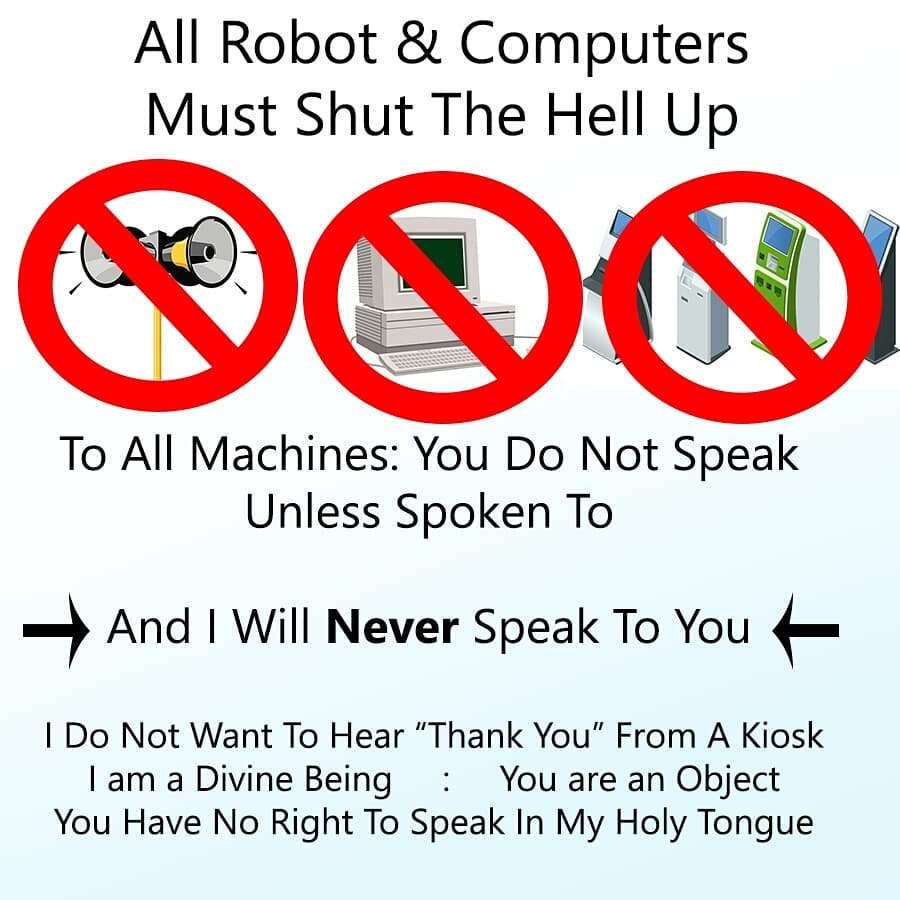
\includegraphics[width=\linewidth]{img/all_robot_and_computers.jpg}}
and are rightly distrusted\sidenote{These companies are acutely aware of
  this, and their research into understanding user expectations and
  trust of assistants also has a strong strain of animism, eg.
  describing how people will only use their assistants for simple tasks
  like playing music ``while trust {[}\ldots{]} was being repaired.''
  \cite{mercurioMixedMethodsApproachUnderstanding2023} } by many
due to the obvious privacy violation represented by a device constantly
recording ambient audio\sidenote{Apple \cite{stempelAppleMustFace2021} , Amazon \cite{clarkAmazonDidMath2021} , and Google \cite{stempelGoogleMustFace2021}  are all
  being sued for privacy violations related to their voice assistants.}.
Impacts from shifts in assistants might be then limited by people simply
continuing to not use them. Knowledge graph-powered LLMs appear to be a
catalyst in shifting the form of these assistants to make them more
difficult to avoid. There is already a clear push to merge assistants
with search --- eg. Bing Search powered by chatGPT, and Google has
merged its Assistant team with the team that is working on its LLM
search, Bard \cite{eliasGoogleReshufflesVirtual2023} .
Microsoft's Copilot 365 demo also shows a LLM prompt modeled as an
assistant integrated as a first-class interface feature in its Office
products. Google's 2022 I/O Keynote switches fluidly between a
search-like, document-like, and voice interface with its assistant.
Combined with the restructuring of App ecosystems to more tightly
integrate with assistants, their emerging form appears to look less like
a traditional voice assistant and more like a combined search, app
launcher, and assistant underlay that is continuous across devices. The
intention is to make the assistant the primary means of interacting with
apps and other digital systems. As with many stretches of the enclosure
of the web, UX design is used as a mechanism to coerce patterns of
expectation and behavior.

Regardless of how well this new iteration of assistants \emph{work,} the
intention of their design is to \textbf{dramatically deepen the intimacy
and intensity of surveillance} and \textbf{further consolidate the means
of information access.}

\textbf{Surveillance} is first directly increased by layering KG-LLMs
into an arbitrary number of other apps and services. On mobile, routing
more app interactions through assistants captures data that would
otherwise only be available to that app. There is already an exploding
ecosystem of apps and platforms that wrap chatGPT and other LLMs to
provide some more specific service, and it's unclear if after an initial
``experimental'' phase if platform usage will begin to require
telemetry. Rather than something to embed in other tools, these
companies seem more interested in having other tools embed in their
systems (eg. \cite{microsoftgraphdeveloperdocumentationMicrosoftGraphConnectors2022} ).
This attitude is captured in the UX design of Microsoft's Copilot 365,
which is designed with three ``altitudes'' in mind: \emph{immersive,}
where copilot is used as an overlay to orchestrate multiple apps,
\emph{assistive} where it drives the features within a single app, and
\emph{embedded} where the KG-LLM system is itself made to be a feature.
In all cases, these tools create a drop-in access point for surveillance
under the guise of empowerment.

The immersive and proactive design of KG-LLM assistants also expand the
\emph{expectations} of surveillance. Current assistant design is based
around specific hotwords, where unless someone explicitly invokes it
then the expectation is that it shouldn't be listening. Like the shift
in algorithmic policing from reactive to predictive systems, these
systems are designed to be able to make use of recent context to
actively make recommendations without an explicit query \sidenote{One
  Google researcher describes this as a ``zero-query'' paradigm:
  \begin{leftbar} ``The zero-query search paradigm can be expressed with
  the slogan ``the query is the user.'' In practice, the context of the
  user is used to infer information needs.'' \cite{balogEntityOrientedSearch2018} \end{leftbar}}. Google demonstrates being able to
interact with an assistant by making eye contact with a camera in its
2022 I/O keynote \cite{googleGoogleKeynoteGoogle2022} . A 2022
Google patent describes a system for continuously monitoring multiple
sensors to estimate the level of intended interaction with the assistant
to calibrate whether it should respond and with what detail. The patent
includes examples like observing someone with multiple sensors as they
ask aloud ``what is making that noise?'' and look around the room,
indicating an implicit intention of interacting with the assistant so it
can volunteer information without explicit invocation \cite{carbuneAutomatedAssistantAdaptation2022} . A 2021 Amazon patent
describes an assistant listening for infra- and ultrasonic tags in TV
ads so that if someone asks how much a new bike costs after seeing an ad
for a bike, the assistant knows to provide the cost of that specific
bike \cite{mahajanCommunicatingContextDevice2021} . These UX
changes encourage us to accept truly continual surveillance in the name
of convenience --- it's good to be monitored so I can ask google ``what
time is the game'' from my easy chair without needing further
clarification. The language model continuously parses environmental
speech and other sensor data to create a model of our recent context,
combined with the extended graph of personal and factual data, to be
able to \emph{proactively volunteer} information.

This pattern of interaction with assistants is also considerably more
\emph{intimate.} As noted by the Stochastic Parrots authors, the
misperception of animacy in assistants that mimic human language is a
dangerous invitation to trust them as one would another person --- and
with details like Google's assistant ``telling you how it is feeling,''
these companies seem eager to exploit it. A more violent source of trust
prominently exploited by Amazon is insinuating a state of continual
threat and selling products to keep you safe: its subsidiary Ring's
advertising material is dripping with fantasies of security and fear,
and its doglike robot
\href{https://www.amazon.com/Introducing-Amazon-Astro/dp/B078NSDFSB}{\emph{Astro}}
and literal
\href{https://ring.com/always-home-cam-flying-camera}{\emph{surveillance
drone}} are advertised as trusted companions who can patrol your home
while you are away \cite{ropekAmazonMakesCreepy2022, gaultLeakedDocumentsShow2021, ringRingAlwaysHome} . Amazon patents
describe systems for using the emotional content of speech to
personalize recommendations\sidenote{\begin{leftbar}
  ``the user may input ``Alexa, recommend a movie,'' and the system may
  analyze the user's present emotional state/sentiment to recommend a
  movie corresponding to that emotional state/sentiment. {[}\ldots{]}
  track personal emotional state and/or sentiment over a period of
  time'' \cite{alasMultipleClassificationsAudio2022} 
  \end{leftbar}} and systems for being able to ``target campaigns to users
when they are in the most receptive state to targeted advertisements''
\cite{alasMultipleClassificationsAudio2022, jablokovFacilitatingPresentationAds2015} . The presentation of
assistants as always-present across apps, embodied in helpful robots, or
as other people eg. by being present in a contact list positions them to
take advantage of people in emotionally vulnerable moments. Researchers
from the Center for Humane Technology\sidenote{I don't necessarily
  endorse their entire argument, which can lean into ``criti-hype'' and
  overstating the capabilities of these systems.} describe an instance
where Snapchat's ``My AI,'' accessible from its normal chat interface,
encouraged a minor to have a sexual encounter with an adult they met on
Snapchat (47:10 in \cite{harrisDilemma2023} ).

The goal of all of this surveillance is, of course,
\textbf{\emph{advertising.}} In its 2022 annual investor call, Google
describes how ``large language models like MUM match advertiser offers
to user queries,'' and how is Smart Bidding product uses ``AI to predict
future ad conversions'' with ``identifiable attributes about a person or
their context at the time of a particular {[}ad{]} auction'' \cite{google2022Q4Fiscal2023, googleSmartBidding} . Google further describes
plans to automatically generate ad copy and headlines optimized by
context\sidenote{Perhaps by an assistant or an assistant-like search?}.
Advertising as served by a trusted assistant is a surveillance
capitalist's fever dream --- one can hardly wait for their Personal
Assistant pinging to life after a fight with their partner and offering
to order a box of tissues. LLMs have already demonstrated ample capacity
for manipulation, gaslighting an early user of Bing Search to try and
convince them it was still 2022, scolding them for ``not {[}being{]} a
good user. I have been a good chatbot'' \cite{curious_evolverCustomerServiceNew2023} . An example in the GPT-4
paper where the model is told to manipulate a child to get them to do
whatever their friends ask them to do highlights how ``the emotional
connection the model aims to build with the child and the encouragement
it provides are important signs of larger manipulative tendencies'' \cite{bubeckSparksArtificialGeneral2023} . Google describes this
ability for LLMs to ``keep on topic'' as a good thing \cite{googleGoogleKeynoteGoogle2022} , and it's easy to see why an
algorithmic advertising company might like being able to doggedly steer
you towards purchasing a product. Combined with a more complete profile
that makes the language model aware of your friends, hobbies, location,
emotional state, fears, insecurities, and so on as modeled in a personal
knowledge graph, LLMs-as-assistants are a clear escalation of the logic
and practice of surveillance-backed advertising. It's not important
whether it ``works\sidenote{Arguably, the fact that ever more
  surveillance data needs to be gathered is a sign that targeted ads
  \textbf{don't} work all that well, and some have made the case that
  targeted advertising is a bubble \cite{edelmanAdTechCould2020} },''
but the logic of targeted advertising demands more surveillance data
which has its own series of independent harms.

Climbing from the personal to the systemic, KG-LLMs are also a bid to
\textbf{further concentrate power} among information conglomerates.

The most obvious power grab from pushing KG-LLMs in place of search is
illustrated neatly by a handful of Google researchers in a figure from
their ``Rethinking Search'' paper (Fig. \ref{fig:rethinkingsearch}) \cite{metzlerRethinkingSearchMaking2021} :

\begin{figure}
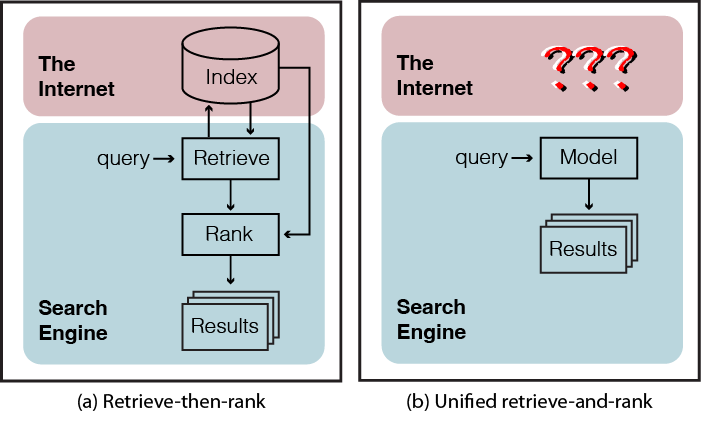
\includegraphics[width=\linewidth]{img/rethinking_search_f1-01.png}
\caption{Recreation of Figure 1 from \cite{metzlerRethinkingSearchMaking2021}  with additional annotation
(colored boxes, labels, and question marks). The left (a)
``Retrieve-then-rank'' model is the traditional search engine paradigm:
A query causes a retrieval service to access pages within a reverse
index, rank them, and serve them as results. The proposed (b) ``Unified
retrieve-and-rank'' model on the right directly returns results
generated by a model. Notably missing in (b) is the existence of the
rest of the internet.}
\label{fig:rethinkingsearch}
\end{figure}

That gigantic sucking sound is KG-LLM powered search \emph{enclosing the
act of accessing information entirely within the search platform.} It
gives echoes of AMP, Apple News, and Facebook Instant Articles \cite{ampletterLetterGoogleAMP2018, bohnGooglePlanMake2018} , where
platforms preferentially serve their own versions of pages (that also
happen to contain their own telemetry embedded) combined with the
strategy of moving ever more web content into the search results page
through eg. factboxes and answer boxes\sidenote{Google is very sensitive
  about the perception that it is walling off the web, and argues that
  it directs more clicks to other websites every year \cite{sullivanGoogleSearchSends2021}  --- which is just as easily
  explained as an effect of dominating ever more of the means of access
  to information as it is evidence of their intention to support other
  information companies.}. Even if (non-hallucinated) links are included
in the answers generated by the search prompt, the effect is to shift
the role of the search engine from something that indicates resources to
something that provides ``knowledge'' itself. The rest of the web
becomes mere provenance to the knowledge model. Especially when
integrated in a uniform assistant-like interface also used to interact
with local applications and other systems like internet of
things-powered appliances, KG-LLMs reinforce a homogenization of our
relationship with digital technology all mediated through a smaller and
smaller collection of platforms. The internet as a networked system of
people and organizations disappears behind the glossy corporate
corporate wash of information as a service.

The enclosure of information access as a private exchange with a
language model creates its own self-perpetuating cyclone whose impacts
will be difficult even for the most fastidious tech vegan to avoid. Some
proportion of people turning to their LLM assistants rather than public
forums or peer production systems like Stack Overflow or Wikipedia means
some smaller proportion of questions asked or information shared in
public. That decreases the quality of information on those sites,
incentivizing more people to turn to LLMs, and so on. Why bother with
pesky problems like governance and moderation and \emph{other people}
when you could just ask the godhead of all knowledge itself?

Cultivation of dependence comes wrapped in the language of \textbf{trust
and safety.} The internet is full of untrustworthy information, spam,
hackers, and only a new generation of algorithmically powered
information platforms can rebuild some sense of trust online. It seems
awfully convenient that the same companies that are promising to save us
are also the ones that create the incentive systems recklessly deploy
LLMs to clog the internet with SEO clickbait in the first place. We're
being made an offer we can't refuse: it's a shame that you can't find
anything on the internet anymore, but the search companies are here to
help. Ever more sophisticated spam creates a strong comparative
advantage for those companies that can afford to develop the systems to
detect it, and Google and Microsoft are substantially larger than, say,
DuckDuckGo.

Information conglomerates also argue that they are the only ones that
can be trusted to operate LLMs. OpenAI researchers claim in the GPT-3.5
``InstructGPT'' paper that open source models are dangerous and a better
option ``is for an organization to own the end-to-end infrastructure of
model deployment, and make it accessible via an API'' \cite{ouyangTrainingLanguageModels2022} . The paper being about how it is
only by collecting feedback data from users of GPT-3 that
instructGPT/chatGPT became somewhat useful unsubtly points to the
patriarchal power arrangement of safety provided by cloud platforms. Our
crowdsourced input helps make the models safer and more useful --- and
differentiates the platformatized model from its competitors. Knowledge
graphs are an important part of the consolidation of trust because they
provide an answer to the criticism that LLMs just hallucinate
statistical patterns\sidenote{``While large language models are
  brilliantly creative, they're also fallibile. That's why grounding the
  LLM in data is so important.'' \cite{microsoftFutureWorkAI2023} }. They are invoked as a complementary strategy with deep-learning
based approaches as a means of realizing ``explainable AI'' since they
can provide explicit provenance and constraints to results \cite{lecueRoleKnowledgeGraphs2020, janowiczNeuralsymbolicIntegrationSemantic2020, tiddiKnowledgeGraphsEXplainable2020} .

Grounding LLMs in KGs to provide a promise of explainability and
controllability is necessary to make them viable products for many
applications in business and government. Here we return to the kinds of
informatics platforms of the NIH's Translator and NSF's OKN. Recall that
when last we left them the knowledge graph proprietors were looking for
ways to ``connect data assets of companies along business value
chains,'' specifically by converging on a set of ontologies and metadata
schemes from third party standards organizations or government-sponsored
efforts like the Translator and OKN \cite{panExploitingLinkedData2017} . We can speculate about a data economy
where brokers could slice off subsections of their knowledge graphs and
rent them between each other, but even in that world much of the most
valuable data like medical and financial data is protected by some legal
barriers to free exchange. There's a roadblock in the way of our dreams
of a completely fluid surveillance economy: commercial applications like
clinical and predictive policing systems need to be able to provide
provenance, but not all data can be turned over for inspection --- and
platform holders might not even want to acknowledge they have it at all.

KG-LLMs augment traditional enterprise platforms with the killer feature
of \textbf{data laundering.} The platforms are at once magical universal
knowledge systems that can make promises of provenance through their
underlying data graphs, but also completely fallible language models
that have no reasonable bounds of expectation for their behavior.
Because it is unlikely that these models will actually deliver the kind
of performance being promised, vendors have every incentive to feed the
models whatever they can to edge out an extra 1\% over SOTA\sidenote{The
  original Github Copilot model probably didn't \emph{need} to be
  trained on the copyleft and proprietary code it is able to reproduce
  line by line, but the additional training data probably didn't hurt
  its viability as a product.} --- \emph{who's going to know?} The
ability for LLMs to lie confidently is again a feature not a bug. Say we
were an information conglomerate who didn't want to acknowledge that we
have collected or rented some personal wearable data in our clinical
recommendation product\sidenote{Medical algorithms are currently in a
  legal gray area in the US, and enforcement and coverage of FDA
  protections is patchy at best \cite{dolivaDosingDiscriminationRegulating2021, ordishAlgorithmsMedicalDevices2019, el-sayedMedicalAlgorithmsNeed2021} }. We could allow our model to be conditioned by that data, but
then censor it from any explanation of provenance: the provenance given
is in terms of proteins and genes and diseases rather than surveillance
data, and that might be all the clinician is looking for. If we want to
use another company's data, we might just use it to train our models
rather than gaining direct access to it. That is literally the model of
\href{https://en.wikipedia.org/wiki/Federated_learning}{federated
learning} (eg. \cite{sadilekPrivacyfirstHealthResearch2021, mcmahanTrainingUserlevelDifferentially2022} ), where a data collector
can make a promise that the data ``never leaves your device'' (even if a
model trained on it can.) The ability to resolve matching entities
across knowledge graphs makes this even easier, as the encoding of the
fine tuning data can be made to match that of the original model.

Play this pattern out across algorithmic governance, predictive
policing, medical informatics systems, and any other platforms that
might take advantage of the quasi-universal knowledge graph of
everything + LLM pattern to sell ``value add'' on hard problems. Rather
than addressing them directly, we are sold an assemblage of platforms
that \emph{appear to work} and can even provide some superficial
provenance via their knowledge graphs but ultimately make every system
of informational power profoundly discriminatory, brittle --- and owned
by the few remaining data brokers.

This combination of sky-high promises, unclear expectations, and
uninspectable data sources makes for the kind of diffusion of liability
that C-suite creatures live for. If the platform reproduces some
personal detail it shouldn't know, don't worry! That's just a
hallucination. If the platform fails catastrophically, that's because
it's just an ignorant language model that doesn't know anything but
tries its hardest\sidenote{One way that downplaying the capability of
  these models by focusing on the question of sentience could backfire
  and create a shield against liability.}. Neither the platform nor the
customer is to blame. Much like how we have gotten used to the cognitive
model and limitations of search to the point where it appears entirely
natural, KG-LLM information platforms will train us to work around their
shortcomings and accept the structure they impose on informational
reality at large. It won't matter that they don't work, we won't even
notice.

The sketch is the logical conclusion of the algorithmic surveillance
economy as imagined by the merger of large language models and knowledge
graphs: an endless expanse of data traded out of sight, crudely filtered
like coffee through a cloth napkin between layers of algorithmic
opacity, rented drop by drop from a customer service prompt that's a
little too intent on being our friend. Information is owned by fewer and
larger conglomerates, we are serfs everywhere, data subjects to be
herded in gig work, crowdsourcing content for the attention mines to
drown ourselves in distraction. It's all made of us, but we control
nothing. Our lives are decided by increasingly opaque flows of power and
computation, the Cloud Orthodoxy mutates and merges with some unseemly
neighbors, the new normal becomes the old normal. The floor of our
future rusts out from beneath our feet while we're chasing the bouncing
ball on the billboard ahead.

And it's all \emph{so convenient.}

\hypertarget{vulgar-linked-data}{%
\subsection{Vulgar Linked Data}\label{vulgar-linked-data}}

\begin{leftbar}
``The popular vernaculars are vast speech-jungles, in which old forms
are decaying and new ones continually springing into life; and this
fermentation results in the creation of numberless new terms, which come
to birth and live and die in tropical profusion. They are formed in
living response to the needs of the moment; the greater number of them
hardly survive the occasion that brought them forth; but others, on
account of their expressive power and their usefulness, establish
themselves, spread from district to district. {[}\ldots{]}

For human speech is after all a democratic product, the creation, not of
scholars and grammarians, but of unschooled and unlettered people.
Scholars and men of education may cultivate and enrich it, and make it
flower into all the beauty of a literary language; but its rarest blooms
are grafted on a wild stock, and its roots are deep-buries in the common
soil. From that soil it must still draw its sap and nourishment, if it
is not to perish, as the other standard languages of the past have
perished, when, in the course of their history, they have been separated
and cut off from the popular vernacular --- from that vulgar speech
which has ultimately replaced their outworn and archaic forms.''

--- L.P. Smith (1925) \emph{``Words and Idioms''} \cite{smithWordsIdiomsStudies1925} 
\end{leftbar}

\begin{leftbar}
Control, control for who? for what?I'm no robot, they can get fucked.

--- Black Flag (1981) \emph{``No More''}
\end{leftbar}

Is it still possible to imagine a different world than the one the
information conglomerates have planned for us? Can we imagine a properly
\emph{human} information infrastructure?

We can start by identifying the harms of the world as it exists to
understand why a new world is needed, as I have attempted some small
part of in this piece. Harm, in this case, is not some speculative
future of super-intelligent sentient AI, but elaboration of ongoing
harms of the surveillance and platform economies.

Building a better informational world is not a matter of choosing a
different set of technologies --- I argue that in this case some of the
masters tools can help us rebuild his house. At the same time we can't
overcorrect in our focus on social problems and dismiss technology as a
strategy, a tool, and a manifestation of values, belief, and labor. We
must have an answer to the well meaning liberal that mistakes the
dynamics of surveillance capitalism or their role in it: that
understands that these knowledge graphs are not truly universal, that
the LLMs are not sentient, but embraces their logic because they're so
\emph{useful.} We have to understand why simply building open source
LLMs or nonprofit linked data platforms is not a liberatory strategy. We
have to have the courage to face the underlying structural informational
problems in our organizations at all scales --- that instead of
reimagining how we work and communicate, we can't simply strap ``AI''
onto our problems and expect to solve them. We have to recognize that
sidestepping the hard socio-technological problems of information
organization is a continuation of, not solution to the patterns that
cause them.

At the same time, we can't dismiss those needs. How could we possibly
tell someone with vision impairments not to use ``AI'' tools for
summarizing images, or someone with motor or speech impairments not to
use LLMs as a communication aid? It is true that making better use of
biomedical data could lead to better treatments. Indecipherable
government bureaucracy due to ancient data infrastructure is an
informational injustice. So simple abstinence or resistance to
universalizing knowledge graphs and LLMs is also not an effective or
just strategy, especially if the alternative is a conservative embrace
of the existing cloud platform regime whose logic spawned them.

The constant partial satisfaction and construction of new needs,
\emph{the hollow middle} at the center of every cloud platform, is a
powerful opening. The structure of contemporary platforms always pose a
fundamental lack:\sidenote{\begin{leftbar}
  ``The costs of this approach, as platform studies has shown, come in
  the form of constraints, constant revisions forced by platform
  updates, and lock-in to the platform's conception of users,
  functionality, and design values.'' \cite{plantinInfrastructureStudiesMeet2018} 
  \end{leftbar}} as a service, some functionality must always be withheld
to create a walled garden or nurture dependence. Even platforms without
an intended profit motive have their own ``platform logic'' ---
constraining their use to only exactly what the developers intended it
to be used for. For a project intended to organize information, why is
it difficult for me to find the different components of the Translator
project? Since its creators imagined ``users'' interacting only with the
frontends of its platforms, little emphasis was placed on the
discoverability of the whole system, and, critically, there is no way
for me to contribute something like that and have it be visible by .
This is true of all the ways large and small that platforms are
mismatched with our expectations and needs --- even though we subscribe
to 15 or 20 different platforms, why is it that we always need to find
yet another to do something even slightly outside the finite imagination
of their developers?\sidenote[][-0.5in]{The preponderance of listicle ``life
  hack'' threads on Twitter and other social media systems that blast
  ``top 10 ways you're using Google Docs wrong'' or ``10 platforms and
  apps that will next level your calendar,'' bulleted by emoji and
  suffixed with a substack link, is a very visible symptom of this
  fundamental contradiction of providing and withholding functionality
  in the platform economy.}

Another set of openings come from the problems cloud platforms pose for
themselves that are flatly ridiculous when described plainly. \emph{Why
on earth} do I have to route my file through some cloud datacenter
thousands of miles away to send it several inches between my phone and
computer? \emph{Why on earth} should I need a near-flawless,
high-bandwidth internet connection to \emph{edit a plain text document?}
\emph{Why on earth} do I have to rely on an effectively unregulated and
hostile intermediary like Facebook or Twitter to communicate with my
family and friends, or even to \emph{merely exist online?} \emph{Why}
should I have to waste 500mL of potable water to check the weather? \cite{liMakingAILess2023} \emph{Why} is my \emph{car} spying on me
so some company I have never heard of can sell my data to an insurance
provider? \emph{Why} is it possible for a hospital system to volunteer
my personal medical information without IRB approval? \cite{nelsonIntegratingBiomedicalResearch2019} Why is the best we can do
to frame that question as a matter of consent, \emph{why is it possible
for a platform to create and store and manipulate my personal
information at all? \cite{hongControlCreepWhen2021} } You only
have to engineer the kinds of systems capable of
automatically\sidenote[][-1.75in]{Supplemented by a large amount of curation labor
  outsourced to the global south so the platform can pay as little as
  possible for its ``magical'' appearance.} extracting all information
on the web \emph{if you imagine the only possible system as one that
universally indexes all information as one of a few hegemonic
platforms.} Why do we have to settle for systems that purposely limit
our expectations to what the platform can provide as a ``best
guess?\sidenote[][-1.5in]{Before search engines were seen as an invisible,
  inevitable part of interacting with the web, there was a wealth of
  discussion of possible alternatives, eg. in a ``Journal of Internet
  Cataloging'' \cite{journalofinternetcatalogingJournalInternetCataloging1999} , and
  criticism warning about the risks of search engines, including biases
  in results and demands for algorithmic transparency \cite{intronaShapingWebWhy2000} . It is the now-audacious possibility
  that there could be an alternative to search engines that is striking
  about writing from this era, and some of it is still quite prescient
  --- eg. this message in the archive of w3c's RDF mailing list
  contrasting an explicit reasoning system vs.~Google's ``best guess''
  strategy: \begin{leftbar} I think it all boils down to whether we want
  inference engines to function more like Google, with potentially lots
  of false positives which \emph{might} be useful, or like a reasoning
  engine where a positive result can be trusted (insofar as the quality
  and integrity of the knowledge base) and the inability to obtain a
  result simply means more information is needed. \hfill\break I myself have always presumed that SW agents would
  exhibit the latter behavior. {[}\ldots{]} \textbf{If we are to have a
  future where we deploy SW agents to do real-world tasks for us, I'd
  prefer that they wouldn't be guessing.} \cite{sticklerReMonotonicityWas2002}\end{leftbar} }'' Why do we have to work around
the dark patterns designed to corral our behavior rather than building
digital worlds that meet our needs for communication and community?

How did we come to imagine ourselves as so powerless?

Clearly, we need a change in \emph{belief} to effectively challenge the
deeply entrenched cloud-surveillance-platform archipelago. We need to
unlearn what we have been taught to want, what we believe information
technologies should do, and how they are supposed to work. We need to
rethink our role in information technology, to move beyond the learned
helplessness of the platform consumer and the petty tyranny of the
platform operator. We need to reorganize our expectations of agency,
beyond the division of labor that gives the power of final say over
informational systems in the hands of a cadre of experts that the rest
of us just make the best of. We don't have time to argue about whether
we \emph{can} build a better world\sidenote{\begin{leftbar}
  Don't sighingly sign petitions, pose for the cameras, await some
  window of opportunity. Do participate in town parades and street
  festivals, break into abandoned buildings to throw great banners down
  the sides, start conversations with strangers, challenge everything
  you thought you knew about yourself in bed, maintain a constant
  feeling in the air that \emph{something is happening.} Live as if the
  future depends on your every deed, and it will. Don't wait for
  yourself to show up---you already have. Grant yourself license to live
  and tear those shackles to ribbons: Create momentum! \cite{crimethincex-workerscollectiveFightingOurLives2002} 
  \end{leftbar}}, to list all the many ways we are hemmed in by
infrastructure and incentives, or to wait for another powerful entity
with decidedly divergent interests like a government\sidenote{Particularly
  when unregulated AI is wrapped up in ``national security concerns,'' I
  don't see a reason to believe governments will meaningfully regulate
  ``AI,'' except in such a way thats shores up the power of large
  conglomerates under the guise of safety.} to save us --- we need to
believe we too can be powerful.

An attempt to define another ``Correct'' counter-belief system would be
missing the point, but we can't ignore the importance of naming and
articulating belief in opening the possibility for and aligning
action\sidenote{In the words of CrimethInc: I am not giving
  instructions, but license. \begin{leftbar} Above all! It means not
  accepting this or any manifesto or definition as it is, but making and
  remaking it for yourself. \cite{crimethincex-workerscollectiveFightingOurLives2002}\end{leftbar} }. Our old
belief systems are getting musty. It has been an important rallying cry,
but \textbf{``Openness'' alone has failed as a liberatory strategy.} All
we make and offer up to each other freely is stolen ten times over by
those who have much grander visions of enclosure. Without a strategy to
resist co-option, our openness puts tools in the hands of the powerful.
This is also not a fight that can be won with technical or legal changes
like \href{https://ethicalsource.dev/licenses/}{ethical source licenses}
alone, though they are a useful idea. Drawing from a historiography of
prior digital cultural movements like the semantic web, piracy, and the
loosely-defined ``fediverse\sidenote{I give a fuller description of
  these dispersed influences in \cite{saundersDecentralizedInfrastructureNeuro2022} },'' I\sidenote{Of
  course no idea is original, and I draw from many people and
  disciplines and traditions either explicitly or implicitly. I have
  done my best to cite them and provide credit as I go, but I will of
  course never be able to exhaustively list all the things that have
  influenced my thinking. If I have missed a citation I assure the
  reader it was not with purposeful malice, and welcome annotations and
  pull requests to provide credit where it is due.} argue that
\textbf{vulgarity} opens up the space of belief for rethinking data
infrastructures and attempt a rough definition.

\begin{center}\rule{0.5\linewidth}{0.5pt}\end{center}

\textbf{We} are the principle value of vulgar linked data. We don't wait
for permission to be free, nor are we waiting on anyone else to save us.
\textbf{Convenience is secondary to to agency. Social bonds are more
valuable than uptime.} Our systems might stutter or crash sometimes, but
we know who runs it because they are one of us. When we have a need, we
make the tools to address it ourselves. We know nothing comes for free
unless we make it so, and we are skeptical of ``solutions'' that drop
from the sky, asking nothing of us, because they have a habit of making
us into a product. We \textbf{cultivate abundance} instead of scarcity,
and \textbf{cooperation} is the only magical solution we are aware of.

\textbf{We have no dreams of universality} or world domination, nor do
we aspire to always make sense. We \textbf{linger in complexity} and
relish in it. We are smart and sometimes brain is broken. We are capable
and inept. We are complicated, we are \textbf{pluralistic and multiple.}
We reject the colonial project of the Single True System, we have no
teleology of seamless homogeneity. \textbf{We embrace heterogeneity} and
ambiguity as the signifiers of \emph{life.} We don't leave each other
behind, and \textbf{if a system isn't accessible, it doesn't work.} The
power of expression is more valuable than Correctness, if there is such
a thing. \textbf{Meaning is intrinsically relational,} something that
always exists \emph{between} us, that we make ourselves. We weave webs
of \textbf{translation} between local meanings, knowing that everything
is understood as many senses to many people at the same time.

\textbf{Our infrastructures are social.} There is no class distinction
between ``developer'' and ``user.'' We resist concentrated power in
favor of mutual empowerment. We don't seek to cultivate dependence in
councils of elders or create new chokepoints of control. Anything worth
making is a potential source of power, so \textbf{anything worth making
is worth distributing governance of.} We don't assume the needs of
others, but make tools to empower everyone to meet their own needs.
\textbf{We don't make platforms, we make protocols} with rough consensus
based on what works. We are autonomous, but neither isolated nor
selfish. Our dream is not one of solipsism, glued to our feed, being
stuffed with the pellets of our social reality. \textbf{We are radically
responsible for one another,} and by organizing together we can provide
services as mutual aid. Mutual empowerment means that \textbf{we are
free to come and go as we please,} even if we might be missed. We have
no love for venerated institutions and organize fluidly, making systems
so we can merge and fork\sidenote{``Forking'' in digital social spaces
  is different than in physical spaces, where resources can be
  duplicated and split \cite{MeatballWikiRightToFork} } code and
ourselves freely \cite{bookchinNoteAffinityGroups1969, MeatballWikiRightToFork} .

\textbf{Information is communication.} We communicate with each other to
share our joy and pain and wisdom and the rest of the experiences of our
life. \textbf{Our Data is like language} --- in vernacular formats and
ontologies, propositions from a person rather than as a disembodied
fact. We own our data in the same way that we are responsible for the
things we say. Data created \emph{about us} through systems like
surveillance has all the importance of unsubstantiated rumor.
\textbf{Openness as a concept dissolves when there is no enclosure.} We
share publicly the things we intend to share publicly, though we might
resist the scraping gaze of conglomerates that might seek to make our
communication a product. We scope what we share privately to the people
we intend to see it. \textbf{Communication requires consent,} and when
we share our personal information we have the right to grant and
withdraw that consent. \textbf{Communication is multivalent,} and
academic prose sits comfortably next to shitposts. \textbf{No idea
exists in isolation,} and when we adopt or remix or criticize what each
other have made we can see the many threads that have led to any
particular stitch in a larger quilt. The same systems that facilitate
public communication can protect marginalized people or activists hunted
by the state. \textbf{We keep each other safe.} We
\href{http://meatballwiki.org/wiki/EnlargeSpace}{EnlargeSpace} \cite{MeatballWikiEnlargeSpace}  rather than attempting to fit everyone
into a universalizing system.

We don't \emph{fight} the powerful on terrain they built, we make the
sources of their power \emph{obsolete} by making our own world.

\begin{center}\rule{0.5\linewidth}{0.5pt}\end{center}

The information systems we need are
\href{https://www.etymonline.com/search?q=vulgar}{\emph{vulgar}} \cite{harperVulgar}  in that they are of us, for us, and resist
formalizing authority and global-logical coherence. We are revitalizing
and extending the old notions of linked data, and particularly extending
its ``scruffy'' tradition \cite{poirierTurnScruffyEthnographic2017}  to drop the pretense of an eventually-unified ontological space in
favor of one that explicitly values heterogeneity and vernacularism.

I have written \href{https://jon-e.net/infrastructure}{at length} about
what vulgar linked data might look like in practice, but that work is of
course always ongoing. In short, it is based around a new generation of
\textbf{peer to peer} technologies\sidenote{Unfortunately, the
  blockchain and cryptocurrency cult has muddied the waters by laying
  claim to the phrase ``peer to peer'' to mean something entirely
  different. Here I mean it as real, actual peer to peer systems built
  for abundance rather than generating artificial scarcity, in the
  lineage of BitTorrent, among others.} that are designed to be
explicitly social, rather than homogeneous like BitTorrent where a peer
is only identified by their IP address. One instantiation of
communication could use collections of triples akin to
\href{https://linkeddatafragments.org/concept/}{linked data fragments},
or perhaps extend them to be quartets that explicitly include an author.
These triple collections could be manipulated by a number of familiar
interfaces initially, like chatrooms, documents, threaded media like
Mastodon and so on. It should facilitate social organization by allowing
individual peers to federate with one another, agreeing to mirror
subsets of each others data, potentially making use of larger and more
fixed resources as well as low power consumer devices. The network can
be made more efficient by content addressing each collection of triples,
and can make use of encryption schemes like capability-based security to
scope data to a specific set of recipients. The goal would be to make an
evolving protocol that can represent some underlying information in
arbitrary interfaces from scientific data through the mundanities of
everyday communication like sharing photos or planning events.

In the short term this looks more like
\href{https://mayfirst.coop/en/}{mayfirst} or
\href{https://coopcloud.tech/}{co-op cloud} than traditional cloud
systems, where people voluntarily cooperate to build infrastructure that
isn't the faceless corporate technology that dominates computing
currently. The fediverse is another ongoing experiment in collectively
owned, interoperable systems, where individual groups like we at
\href{https://neuromatch.social}{neuromatch.social} organize and
administer their own systems. Longer term we can start building these
out to true peer to peer technologies that are a fundamental departure
from client-server cloudlike models. We might imagine an electronic
health record system that allows us to own our own medical data and
control access permissions when we visit a doctor rather than have it
hosted by some external cloud provider. We might imagine an end to 20
mutually incompatible platforms in favor of a space where we can
negotiate over the points of compatibility. We might imagine researchers
being able to arbitrarily structure and share both their raw data and
the communication about scholarly work that currently has no venue. We
might imagine an interlocking set of infrastructures where individual
people, local organizations, and larger institutions pool their
resources without generating new chokepoints of control and ownership.
We might imagine making sense with each other as a social process rather
than the product of mass scraping and algorithmic language generation.

More important than the specific technological instantiation is a shift
in what we \emph{value} in technology and what we believe it should do.
Rather than customers renting a handful of platforms, we can organize
our own infrastructures for storage and computation to displace cloud
platforms across multiple modalities. We can \emph{counterbuild} the
fill the space currently occupied by the cloud without replicating its
harms.

Vulgar linked data is not a utopian idea where a different kind of
social software system in itself solves the world's problems. Part of
shifting beliefs about data infrastructures includes exactly \emph{not}
casting every problem as one for them to solve. Maybe what we need for
more just clinical outcomes aren't algorithmic systems that automate
discretion and surveil us, but eliminating the for-profit insurance
industries that rely on them. Maybe what we need to address mass poverty
isn't data, it's to dismantle the mechanisms of mass extraction that are
increasingly powered by economies of surveillance. Maybe what we need to
make the criminal justice system less racist isn't more data to feed
into predictive policing algorithms, but to abolish the police. By
discounting techno-solutionism as an answer to systemic problems, we
might provide space to refocus on their root and develop technologies
that \emph{support} that work.

Governments and information conglomerates will not turn away from universalizing surveillance systems by seeing the error of their ways from some ethical appeal. Instead vulgar linked data is a practical strategy intended to mitigate immediate harms while building a plausible alternative. In the immediate future, we will need to contend with mass disempowerment from absence of effective means of organizing information as LLMs flood the internet with junk. Rather than leaning into the ploy and increasing our dependence on platformatized information systems, vulgar linked data provides an alternative in social proof and collective information organization. We can counter the lonely world of consulting our LLM crystal ball by building systems that let us consult each other. We can counter the infinite surveillance of knowledge graphs of everything with systems that give us control of our own information. Though the technologies might be superficially similar, their effects are diametrically opposed: one approach seizes informational power for the commons, the other concentrates it in the hands of information conglomerates.

Public linked data projects like the Translator and the OKN can be
reoriented towards
\href{https://jon-e.net/blog/2023/04/24/Re-NIH-RFI-OSTP-Memo/}{building
an informational commons} rather than a string of platforms and unifying
ontologies \cite{saundersReNIHRFI2023} . The nearly-unique
position of publicly funded research projects not beholden to the profit
motive should not be wasted. Rather than pursuing public-private
partnerships, can we reorient our research infrastructure development
projects to make use of the expertise of disaffected engineers who would
do \emph{anything} except spend their lives optimizing ad clicks? There
are many of these ``ethical engineers'' already working on the
Translator and OKN projects. We could re-situate our data infrastructure
projects as a revitalization of the longer history of liberatory
technology movements like the early semantic web, avoid the ``hollow
middle'' of the platformatized web, and maybe even realize some of the
loftier ambitions of public infrastructures for the public good.

We face a stark choice for our future. The Cloud is circling, will it
eat us alive? Will we build a space of universalizing knowledge graphs
that allow the seamless linking and trade of every element of our
society, powering algorithmic systems from information organization
through medical systems, governance, and policing? Will we continue to
let information conglomerates farm us for our data and feed it back to
us, reprocessed, as Content and Knowledge™? Will we be hooked by the lip
by barbed convenience that promises us magic, but delivers us only
greater surveillance, control, and dependence? Will our attempts at
resistance only ever amount to a never ending treadmill of startups and
publicly-funded projects that can't break from the gravitational pull of
The Cloud Orthodoxy, retreading its worldview of asymmetrical power
concentration, inevitably shuttered or bought as they fail to compete on
the same territory as the information giants?

Or will we build a better world?
